\documentclass[aspectratio=169]{beamer}
\usepackage{amsmath,amssymb,mathrsfs,fontspec,tikz}
\setsansfont{Liberation Sans}
\setmainfont{Liberation Sans}
\usefonttheme[onlymath]{serif}
\geometry{paperwidth=960.009bp,paperheight=540bp}
\setbeamertemplate{navigation symbols}{}
\setbeamertemplate{headline}{}\setbeamertemplate{footline}{}
\setbeamersize{text margin left=0pt,text margin right=0pt}
\definecolor{ink}{HTML}{242424}
\hypersetup{pdftitle={Research Interview — Yasser Baouzil — KIT},pdfauthor={Yasser Baouzil}}
\begin{document}
\begin{frame}[plain]
\begin{tikzpicture}[remember picture,overlay]
\node[anchor=north west,inner sep=0pt] at(current page.north west){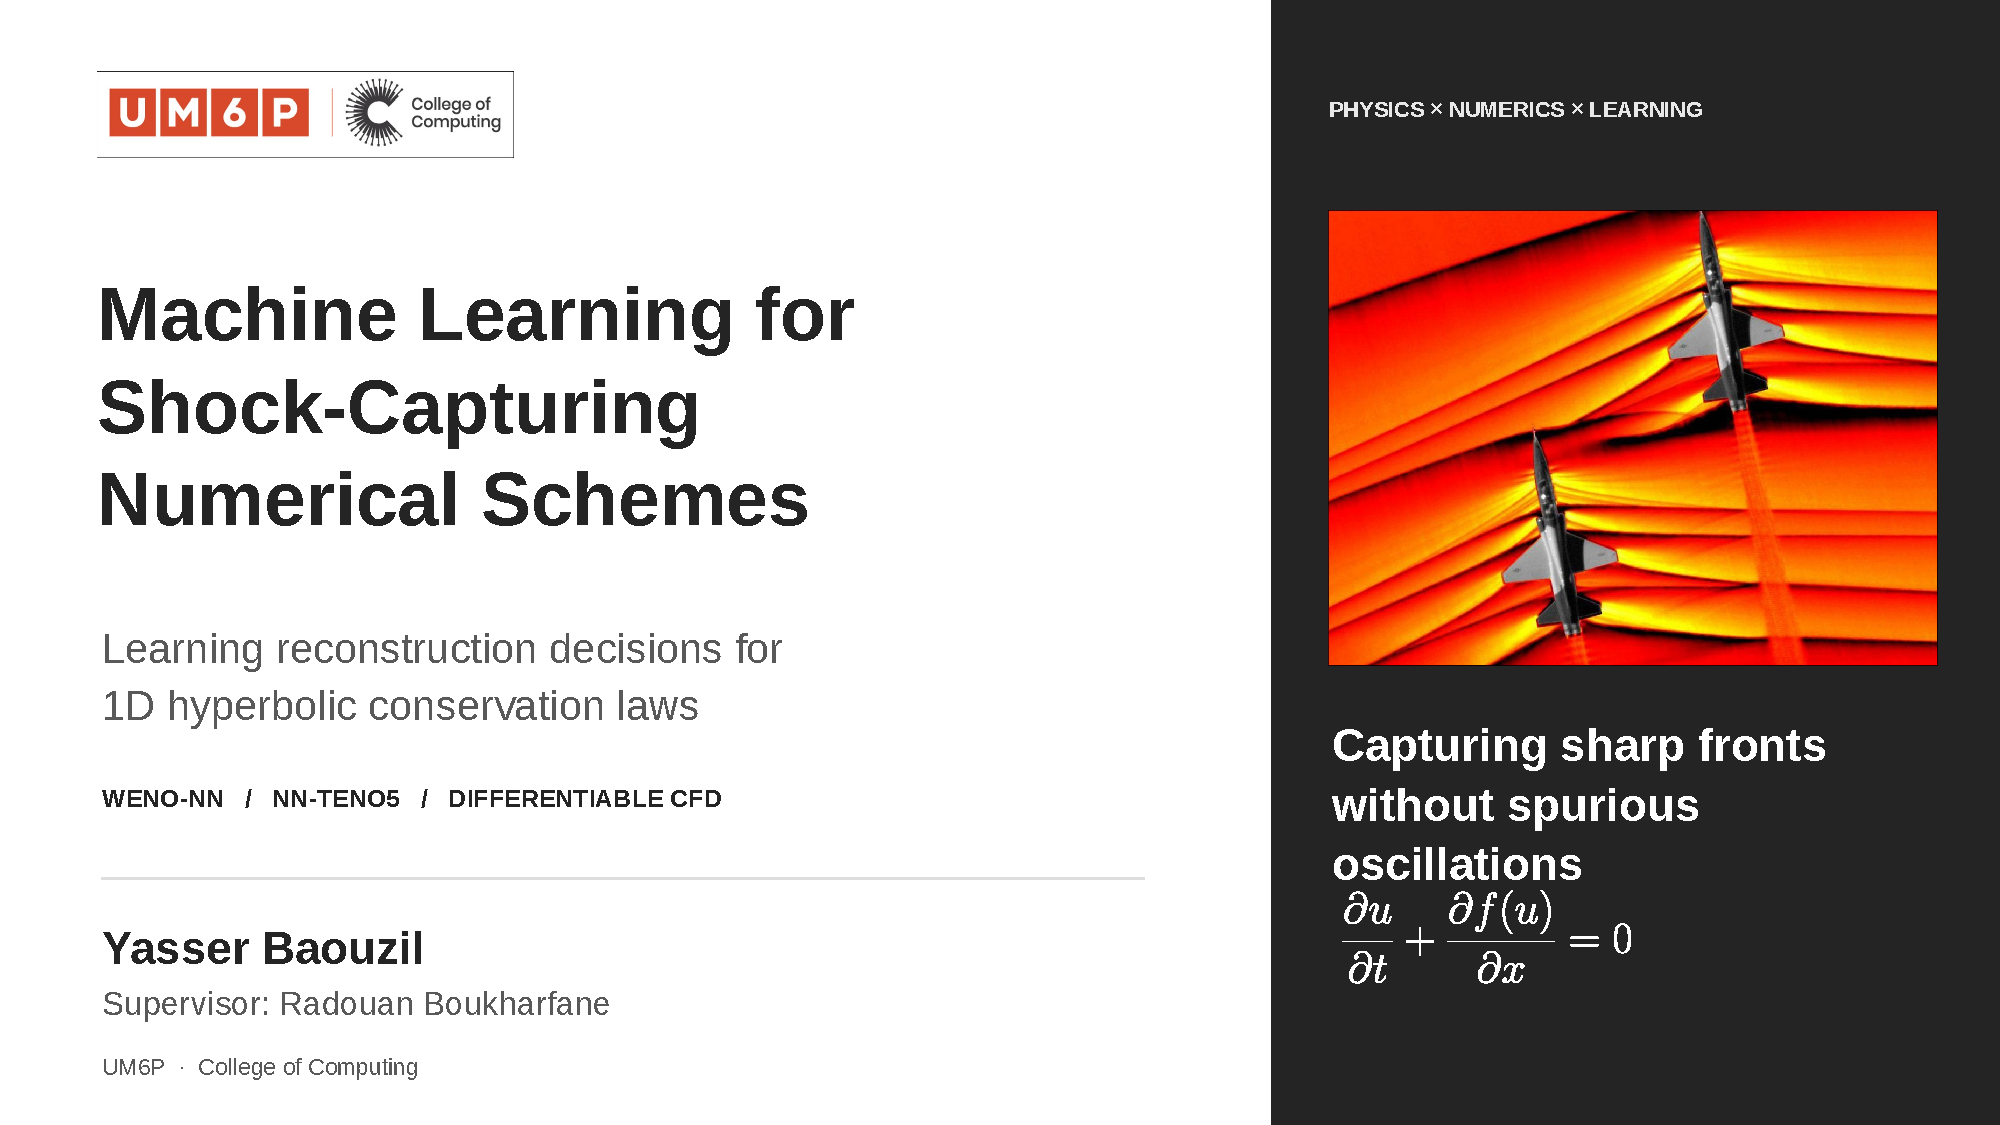
\includegraphics[width=\paperwidth,height=\paperheight]{revised_source/assets/V4_landing-1.pdf}};
\end{tikzpicture}
\end{frame}
% Slide 2: MAIN
\begin{frame}[plain]
\begin{tikzpicture}[remember picture,overlay]
\node[anchor=north west,inner sep=0pt,outer sep=0pt,text={rgb,255:red,36;green,36;blue,36},align=left,text width=10.900000in,font={\fontsize{10.50bp}{11.34bp}\selectfont \bfseries }] at ([xshift=0.600000in,yshift=-0.300000in]current page.north west) {RESEARCH BACKGROUND · SCIENTIFIC MACHINE LEARNING};
\node[anchor=north west,inner sep=0pt,outer sep=0pt,text={rgb,255:red,36;green,36;blue,36},align=left,text width=12.050000in,font={\fontsize{27.00bp}{29.16bp}\selectfont \bfseries }] at ([xshift=0.600000in,yshift=-0.780000in]current page.north west) {Learning inside a classical shock-capturing solver};
\path[fill={rgb,255:red,222;green,222;blue,222},draw=none] ([xshift=0.600000in,yshift=-1.430000in]current page.north west) rectangle ([xshift=12.700000in,yshift=-1.445000in]current page.north west);
\path[fill={rgb,255:red,222;green,222;blue,222},draw=none] ([xshift=0.600000in,yshift=-7.030000in]current page.north west) rectangle ([xshift=12.700000in,yshift=-7.042000in]current page.north west);
\node[anchor=north west,inner sep=0pt,outer sep=0pt,text={rgb,255:red,89;green,89;blue,89},align=left,text width=7.200000in,font={\fontsize{9.00bp}{9.72bp}\selectfont }] at ([xshift=0.600000in,yshift=-7.150000in]current page.north west) {SHOCKS \& WENO   /   YASSER BAOUZIL};
\node[anchor=north west,inner sep=0pt,outer sep=0pt,text={rgb,255:red,89;green,89;blue,89},align=right,text width=1.100000in,font={\fontsize{10.00bp}{10.80bp}\selectfont }] at ([xshift=11.600000in,yshift=-7.120000in]current page.north west) {02 / 9};
\node[anchor=north west,inner sep=0pt] at ([xshift=9.543659in,yshift=-7.120000in]current page.north west) {
\includegraphics[width=1.312683in,height=0.270000in]{revised_source/assets/art_bf8a20b59a0b57.png}};
\node[anchor=north west,inner sep=0pt] at ([xshift=0.633766in,yshift=-1.770000in]current page.north west) {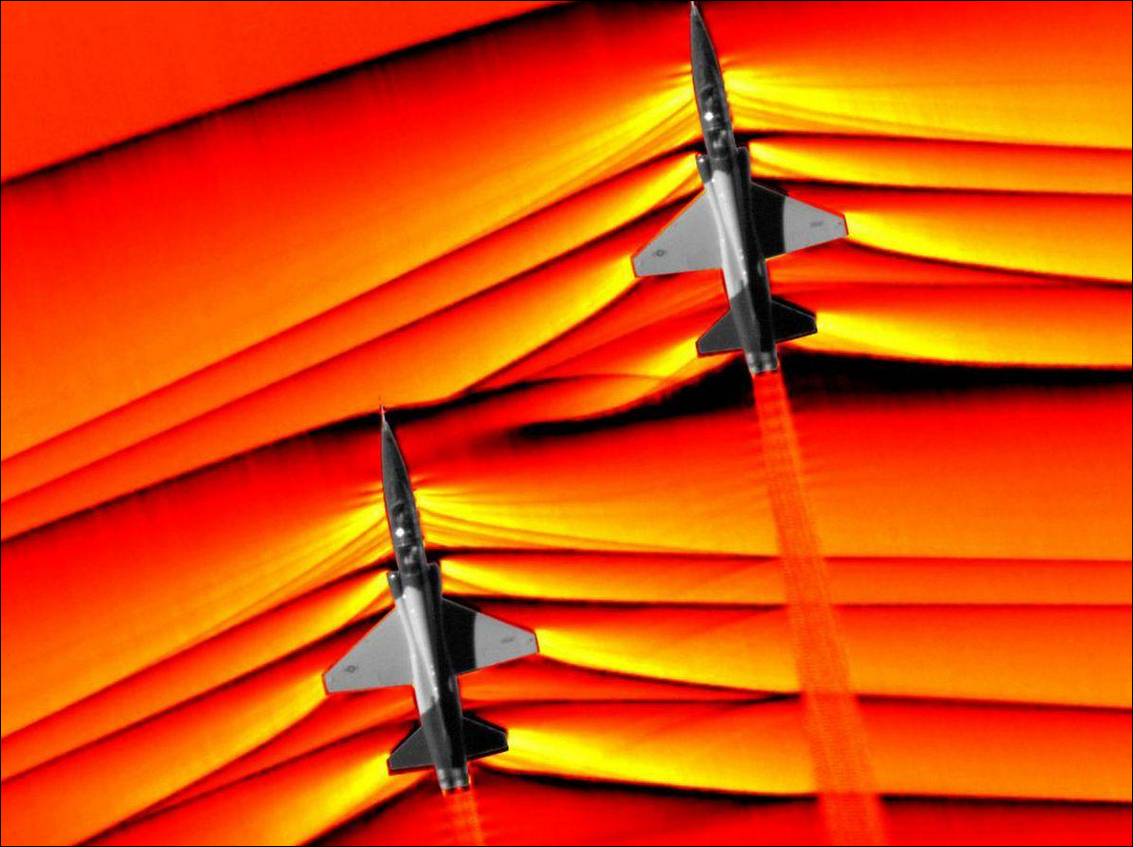
\includegraphics[width=4.882468in,height=3.650000in]{revised_source/assets/art_b38ac0cd5eee7f.png}};
\node[anchor=north west,inner sep=0pt,outer sep=0pt,text={rgb,255:red,36;green,36;blue,36},align=left,text width=6.700000in,font={\fontsize{20.00bp}{21.60bp}\selectfont \bfseries }] at ([xshift=5.940000in,yshift=-1.800000in]current page.north west) {My technical work · scientific-ML internship};
\path[fill={rgb,255:red,245;green,245;blue,245},draw=none,rounded corners=3bp] ([xshift=5.850000in,yshift=-2.390000in]current page.north west) rectangle ([xshift=12.700000in,yshift=-3.430000in]current page.north west);
\node[inner sep=0pt,anchor=center] at ([xshift=7.910139in,yshift=-2.905000in]current page.north west) {\color[HTML]{242424}\fontsize{32.000bp}{38.400bp}\selectfont $\displaystyle \partial_t U+\partial_xF(U)=0$};
\node[anchor=north west,inner sep=0pt,outer sep=0pt,text={rgb,255:red,89;green,89;blue,89},align=left,text width=6.550000in,font={\fontsize{17.30bp}{22.84bp}\selectfont }] at ([xshift=5.960000in,yshift=-3.660000in]current page.north west) {Modular ENO baseline + WENO/TENO 3, 5, 7\\ Convergence checks; Sod / Shu–Osher benchmarks\\ Characteristic Euler + neural stencil decisions\\ Differentiable JAX rollouts; classical/NN blending\\ Controlled investigation of numerical failures};
\path[fill={rgb,255:red,245;green,245;blue,245},draw=none,rounded corners=3bp] ([xshift=0.600000in,yshift=-5.640000in]current page.north west) rectangle ([xshift=3.470000in,yshift=-6.360000in]current page.north west);
\node[anchor=north west,inner sep=0pt,outer sep=0pt,text={rgb,255:red,36;green,36;blue,36},align=left,text width=2.550000in,font={\fontsize{16.00bp}{17.28bp}\selectfont \bfseries }] at ([xshift=0.760000in,yshift=-5.760000in]current page.north west) {Original WENO-NN};
\node[anchor=north west,inner sep=0pt,outer sep=0pt,text={rgb,255:red,89;green,89;blue,89},align=left,text width=2.550000in,font={\fontsize{12.50bp}{13.50bp}\selectfont }] at ([xshift=0.760000in,yshift=-6.060000in]current page.north west) {Coefficient corrections};
\path[fill={rgb,255:red,245;green,245;blue,245},draw=none,rounded corners=3bp] ([xshift=3.680000in,yshift=-5.640000in]current page.north west) rectangle ([xshift=6.550000in,yshift=-6.360000in]current page.north west);
\node[anchor=north west,inner sep=0pt,outer sep=0pt,text={rgb,255:red,36;green,36;blue,36},align=left,text width=2.550000in,font={\fontsize{16.00bp}{17.28bp}\selectfont \bfseries }] at ([xshift=3.840000in,yshift=-5.760000in]current page.north west) {NN-TENO / oracle};
\node[anchor=north west,inner sep=0pt,outer sep=0pt,text={rgb,255:red,89;green,89;blue,89},align=left,text width=2.550000in,font={\fontsize{12.50bp}{13.50bp}\selectfont }] at ([xshift=3.840000in,yshift=-6.060000in]current page.north west) {Candidate selection};
\path[fill={rgb,255:red,245;green,245;blue,245},draw=none,rounded corners=3bp] ([xshift=6.760000in,yshift=-5.640000in]current page.north west) rectangle ([xshift=9.630000in,yshift=-6.360000in]current page.north west);
\node[anchor=north west,inner sep=0pt,outer sep=0pt,text={rgb,255:red,36;green,36;blue,36},align=left,text width=2.550000in,font={\fontsize{16.00bp}{17.28bp}\selectfont \bfseries }] at ([xshift=6.920000in,yshift=-5.760000in]current page.north west) {JAX / unrolled};
\node[anchor=north west,inner sep=0pt,outer sep=0pt,text={rgb,255:red,89;green,89;blue,89},align=left,text width=2.550000in,font={\fontsize{12.50bp}{13.50bp}\selectfont }] at ([xshift=6.920000in,yshift=-6.060000in]current page.north west) {Rollout loss + blending};
\path[fill={rgb,255:red,245;green,245;blue,245},draw=none,rounded corners=3bp] ([xshift=9.840000in,yshift=-5.640000in]current page.north west) rectangle ([xshift=12.710000in,yshift=-6.360000in]current page.north west);
\node[anchor=north west,inner sep=0pt,outer sep=0pt,text={rgb,255:red,36;green,36;blue,36},align=left,text width=2.550000in,font={\fontsize{16.00bp}{17.28bp}\selectfont \bfseries }] at ([xshift=10.000000in,yshift=-5.760000in]current page.north west) {Later V2};
\node[anchor=north west,inner sep=0pt,outer sep=0pt,text={rgb,255:red,89;green,89;blue,89},align=left,text width=2.550000in,font={\fontsize{12.50bp}{13.50bp}\selectfont }] at ([xshift=10.000000in,yshift=-6.060000in]current page.north west) {Classical gate + NN};
\path[fill={rgb,255:red,36;green,36;blue,36},draw=none] ([xshift=0.600000in,yshift=-6.490000in]current page.north west) rectangle ([xshift=0.642000in,yshift=-6.840000in]current page.north west);
\node[anchor=north west,inner sep=0pt,outer sep=0pt,text={rgb,255:red,36;green,36;blue,36},align=left,text width=11.900000in,font={\fontsize{17.00bp}{18.36bp}\selectfont }] at ([xshift=0.770000in,yshift=-6.480000in]current page.north west) {Objective: improve solution accuracy while retaining numerical reliability.};
\node[anchor=north west,inner sep=0pt,outer sep=0pt,text={rgb,255:red,89;green,89;blue,89},align=left,text width=11.950000in,font={\fontsize{8.50bp}{9.18bp}\selectfont }] at ([xshift=0.660000in,yshift=-6.800000in]current page.north west) {Project scope: src/schemes/ · src/core/ · scripts/legacy\_imitation\_training/ · scripts/unrolled\_physics\_loss/};
\end{tikzpicture}
\end{frame}
% Slide 3: MAIN
\begin{frame}[plain]
\begin{tikzpicture}[remember picture,overlay]
\node[anchor=north west,inner sep=0pt,outer sep=0pt,text={rgb,255:red,36;green,36;blue,36},align=left,text width=10.900000in,font={\fontsize{10.50bp}{11.34bp}\selectfont \bfseries }] at ([xshift=0.600000in,yshift=-0.300000in]current page.north west) {NUMERICAL FRAMEWORK · ACTUAL EULER PIPELINE};
\node[anchor=north west,inner sep=0pt,outer sep=0pt,text={rgb,255:red,36;green,36;blue,36},align=left,text width=12.050000in,font={\fontsize{27.00bp}{29.16bp}\selectfont \bfseries }] at ([xshift=0.600000in,yshift=-0.780000in]current page.north west) {Where the network enters the Euler solver};
\path[fill={rgb,255:red,222;green,222;blue,222},draw=none] ([xshift=0.600000in,yshift=-1.430000in]current page.north west) rectangle ([xshift=12.700000in,yshift=-1.445000in]current page.north west);
\path[fill={rgb,255:red,222;green,222;blue,222},draw=none] ([xshift=0.600000in,yshift=-7.030000in]current page.north west) rectangle ([xshift=12.700000in,yshift=-7.042000in]current page.north west);
\node[anchor=north west,inner sep=0pt,outer sep=0pt,text={rgb,255:red,89;green,89;blue,89},align=left,text width=7.200000in,font={\fontsize{9.00bp}{9.72bp}\selectfont }] at ([xshift=0.600000in,yshift=-7.150000in]current page.north west) {SHOCKS \& WENO   /   YASSER BAOUZIL};
\node[anchor=north west,inner sep=0pt,outer sep=0pt,text={rgb,255:red,89;green,89;blue,89},align=right,text width=1.100000in,font={\fontsize{10.00bp}{10.80bp}\selectfont }] at ([xshift=11.600000in,yshift=-7.120000in]current page.north west) {03 / 9};
\node[anchor=north west,inner sep=0pt] at ([xshift=9.543659in,yshift=-7.120000in]current page.north west) {
\includegraphics[width=1.312683in,height=0.270000in]{revised_source/assets/art_bf8a20b59a0b57.png}};
\node[inner sep=0pt,anchor=center] at ([xshift=3.550000in,yshift=-2.510000in]current page.north west) {\color[HTML]{242424}\fontsize{23.234bp}{27.881bp}\selectfont $\displaystyle U=(\rho,m,E)^{\mathsf T},\quad F(U)=\begin{pmatrix}m\\m^2/\rho+p\\m(E+p)/\rho\end{pmatrix}$};
\node[anchor=north west,inner sep=0pt,outer sep=0pt,text={rgb,255:red,36;green,36;blue,36},align=left,text width=5.900000in,font={\fontsize{17.00bp}{18.36bp}\selectfont \bfseries }] at ([xshift=6.650000in,yshift=-1.910000in]current page.north west) {Conservative forward-Euler building block};
\node[inner sep=0pt,anchor=center] at ([xshift=9.030556in,yshift=-2.785000in]current page.north west) {\color[HTML]{242424}\fontsize{24.000bp}{28.800bp}\selectfont $\displaystyle \bar U_i^{n+1}=\bar U_i^n-\frac{\Delta t}{\Delta x}\left(\widehat F_{i+1/2}-\widehat F_{i-1/2}\right)$};
\path[fill={rgb,255:red,245;green,245;blue,245},draw=none,rounded corners=3bp] ([xshift=0.600000in,yshift=-3.570000in]current page.north west) rectangle ([xshift=2.420000in,yshift=-4.510000in]current page.north west);
\node[anchor=north west,inner sep=0pt,outer sep=0pt,text={rgb,255:red,36;green,36;blue,36},align=center,text width=1.670000in,font={\fontsize{16.00bp}{17.28bp}\selectfont }] at ([xshift=0.675000in,yshift=-3.800000in]current page.north west) {Conserved\\ state U};
\node[anchor=north west,inner sep=0pt,outer sep=0pt,text={rgb,255:red,89;green,89;blue,89},align=center,text width=0.235000in,font={\fontsize{16.07bp}{17.36bp}\selectfont }] at ([xshift=2.420000in,yshift=-3.850000in]current page.north west) {→};
\path[fill={rgb,255:red,245;green,245;blue,245},draw=none,rounded corners=3bp] ([xshift=2.655000in,yshift=-3.570000in]current page.north west) rectangle ([xshift=4.475000in,yshift=-4.510000in]current page.north west);
\node[anchor=north west,inner sep=0pt,outer sep=0pt,text={rgb,255:red,36;green,36;blue,36},align=center,text width=1.670000in,font={\fontsize{16.00bp}{17.28bp}\selectfont }] at ([xshift=2.730000in,yshift=-3.800000in]current page.north west) {Roe basis\\ L and R};
\node[anchor=north west,inner sep=0pt,outer sep=0pt,text={rgb,255:red,89;green,89;blue,89},align=center,text width=0.235000in,font={\fontsize{16.07bp}{17.36bp}\selectfont }] at ([xshift=4.475000in,yshift=-3.850000in]current page.north west) {→};
\path[fill={rgb,255:red,245;green,245;blue,245},draw=none,rounded corners=3bp] ([xshift=4.710000in,yshift=-3.570000in]current page.north west) rectangle ([xshift=6.530000in,yshift=-4.510000in]current page.north west);
\node[anchor=north west,inner sep=0pt,outer sep=0pt,text={rgb,255:red,36;green,36;blue,36},align=center,text width=1.670000in,font={\fontsize{16.00bp}{17.28bp}\selectfont }] at ([xshift=4.785000in,yshift=-3.800000in]current page.north west) {LF split\\ fluxes};
\node[anchor=north west,inner sep=0pt,outer sep=0pt,text={rgb,255:red,89;green,89;blue,89},align=center,text width=0.235000in,font={\fontsize{16.07bp}{17.36bp}\selectfont }] at ([xshift=6.530000in,yshift=-3.850000in]current page.north west) {→};
\path[fill={rgb,255:red,245;green,245;blue,245},draw={rgb,255:red,36;green,36;blue,36},rounded corners=3bp] ([xshift=6.765000in,yshift=-3.570000in]current page.north west) rectangle ([xshift=8.585000in,yshift=-4.510000in]current page.north west);
\node[anchor=north west,inner sep=0pt,outer sep=0pt,text={rgb,255:red,36;green,36;blue,36},align=center,text width=1.670000in,font={\fontsize{16.00bp}{17.28bp}\selectfont \bfseries }] at ([xshift=6.840000in,yshift=-3.690000in]current page.north west) {TENO / NN\\ reconstruction};
\node[anchor=north west,inner sep=0pt,outer sep=0pt,text={rgb,255:red,89;green,89;blue,89},align=center,text width=1.670000in,font={\fontsize{9.80bp}{10.58bp}\selectfont \bfseries }] at ([xshift=6.840000in,yshift=-4.310000in]current page.north west) {LEARNED DECISION};
\node[anchor=north west,inner sep=0pt,outer sep=0pt,text={rgb,255:red,89;green,89;blue,89},align=center,text width=0.235000in,font={\fontsize{16.07bp}{17.36bp}\selectfont }] at ([xshift=8.585000in,yshift=-3.850000in]current page.north west) {→};
\path[fill={rgb,255:red,245;green,245;blue,245},draw=none,rounded corners=3bp] ([xshift=8.820000in,yshift=-3.570000in]current page.north west) rectangle ([xshift=10.640000in,yshift=-4.510000in]current page.north west);
\node[anchor=north west,inner sep=0pt,outer sep=0pt,text={rgb,255:red,36;green,36;blue,36},align=center,text width=1.670000in,font={\fontsize{16.00bp}{17.28bp}\selectfont }] at ([xshift=8.895000in,yshift=-3.800000in]current page.north west) {Shared-face\\ flux};
\node[anchor=north west,inner sep=0pt,outer sep=0pt,text={rgb,255:red,89;green,89;blue,89},align=center,text width=0.235000in,font={\fontsize{16.07bp}{17.36bp}\selectfont }] at ([xshift=10.640000in,yshift=-3.850000in]current page.north west) {→};
\path[fill={rgb,255:red,245;green,245;blue,245},draw=none,rounded corners=3bp] ([xshift=10.875000in,yshift=-3.570000in]current page.north west) rectangle ([xshift=12.695000in,yshift=-4.510000in]current page.north west);
\node[anchor=north west,inner sep=0pt,outer sep=0pt,text={rgb,255:red,36;green,36;blue,36},align=center,text width=1.670000in,font={\fontsize{16.00bp}{17.28bp}\selectfont }] at ([xshift=10.950000in,yshift=-3.800000in]current page.north west) {SSPRK3\\ stages};
\node[anchor=north west,inner sep=0pt,outer sep=0pt,text={rgb,255:red,89;green,89;blue,89},align=left,text width=12.000000in,font={\fontsize{17.00bp}{18.36bp}\selectfont }] at ([xshift=0.680000in,yshift=-4.750000in]current page.north west) {Default path: reconstruct characteristic split fluxes, not physical left/right interface states.};
\path[fill={rgb,255:red,245;green,245;blue,245},draw=none,rounded corners=3bp] ([xshift=0.600000in,yshift=-5.350000in]current page.north west) rectangle ([xshift=8.900000in,yshift=-6.260000in]current page.north west);
\node[inner sep=0pt,anchor=center] at ([xshift=3.475417in,yshift=-5.785000in]current page.north west) {\color[HTML]{242424}\fontsize{29.000bp}{34.800bp}\selectfont $\displaystyle \mathcal R_{V2}=\mathcal R_T+G\lambda\left(\mathcal R_{NN}-\mathcal R_T\right)$};
\node[anchor=north west,inner sep=0pt,outer sep=0pt,text={rgb,255:red,89;green,89;blue,89},align=left,text width=3.420000in,font={\fontsize{15.50bp}{19.38bp}\selectfont }] at ([xshift=9.180000in,yshift=-5.380000in]current page.north west) {Later V2\\ G: classical TENO trouble gate\\ λ: controlled correction strength};
\node[anchor=north west,inner sep=0pt,outer sep=0pt,text={rgb,255:red,89;green,89;blue,89},align=left,text width=11.950000in,font={\fontsize{8.50bp}{9.18bp}\selectfont }] at ([xshift=0.660000in,yshift=-6.800000in]current page.north west) {Implemented: euler\_jax.py:166–254 · gated\_teno5\_jax.py:19–67. SSPRK3 reevaluates reconstruction at every stage.};
\end{tikzpicture}
\end{frame}
% Slide 4: MAIN
\begin{frame}[plain]
\begin{tikzpicture}[remember picture,overlay]
\node[anchor=north west,inner sep=0pt,outer sep=0pt,text={rgb,255:red,36;green,36;blue,36},align=left,text width=10.900000in,font={\fontsize{10.50bp}{11.34bp}\selectfont \bfseries }] at ([xshift=0.600000in,yshift=-0.300000in]current page.north west) {OBSERVED FAILURE · DENSITY AND INTERNAL ENERGY};
\node[anchor=north west,inner sep=0pt,outer sep=0pt,text={rgb,255:red,36;green,36;blue,36},align=left,text width=12.050000in,font={\fontsize{27.00bp}{29.16bp}\selectfont \bfseries }] at ([xshift=0.600000in,yshift=-0.780000in]current page.north west) {Conservation does not ensure positive Euler states};
\path[fill={rgb,255:red,222;green,222;blue,222},draw=none] ([xshift=0.600000in,yshift=-1.430000in]current page.north west) rectangle ([xshift=12.700000in,yshift=-1.445000in]current page.north west);
\path[fill={rgb,255:red,222;green,222;blue,222},draw=none] ([xshift=0.600000in,yshift=-7.030000in]current page.north west) rectangle ([xshift=12.700000in,yshift=-7.042000in]current page.north west);
\node[anchor=north west,inner sep=0pt,outer sep=0pt,text={rgb,255:red,89;green,89;blue,89},align=left,text width=7.200000in,font={\fontsize{9.00bp}{9.72bp}\selectfont }] at ([xshift=0.600000in,yshift=-7.150000in]current page.north west) {SHOCKS \& WENO   /   YASSER BAOUZIL};
\node[anchor=north west,inner sep=0pt,outer sep=0pt,text={rgb,255:red,89;green,89;blue,89},align=right,text width=1.100000in,font={\fontsize{10.00bp}{10.80bp}\selectfont }] at ([xshift=11.600000in,yshift=-7.120000in]current page.north west) {04 / 9};
\node[anchor=north west,inner sep=0pt] at ([xshift=9.543659in,yshift=-7.120000in]current page.north west) {
\includegraphics[width=1.312683in,height=0.270000in]{revised_source/assets/art_bf8a20b59a0b57.png}};
\node[inner sep=0pt,anchor=center] at ([xshift=2.402623in,yshift=-2.090000in]current page.north west) {\color[HTML]{242424}\fontsize{25.491bp}{30.589bp}\selectfont $\displaystyle p=(\gamma-1)\left(E-\frac{m^2}{2\rho}\right)$};
\node[inner sep=0pt,anchor=center] at ([xshift=10.499236in,yshift=-2.100000in]current page.north west) {\color[HTML]{242424}\fontsize{29.000bp}{34.800bp}\selectfont $\displaystyle \rho>0,\qquad p>0$};
\node[inner sep=0pt,anchor=center] at ([xshift=3.336458in,yshift=-2.905000in]current page.north west) {\color[HTML]{242424}\fontsize{25.000bp}{30.000bp}\selectfont $\displaystyle \boxed{\delta p\approx(\gamma-1)\left(\delta E-v\,\delta m+\tfrac12v^2\delta\rho\right)}$};
\node[anchor=north west,inner sep=0pt,outer sep=0pt,text={rgb,255:red,89;green,89;blue,89},align=left,text width=11.600000in,font={\fontsize{13.50bp}{14.58bp}\selectfont }] at ([xshift=0.890000in,yshift=-3.290000in]current page.north west) {v = m/ρ · linearization about an admissible reference state};
\path[fill={rgb,255:red,245;green,245;blue,245},draw=none,rounded corners=3bp] ([xshift=0.600000in,yshift=-3.670000in]current page.north west) rectangle ([xshift=12.720000in,yshift=-4.100000in]current page.north west);
\node[anchor=north west,inner sep=0pt,outer sep=0pt,text={rgb,255:red,36;green,36;blue,36},align=left,text width=5.600000in,font={\fontsize{15.70bp}{16.96bp}\selectfont \bfseries }] at ([xshift=0.800000in,yshift=-3.770000in]current page.north west) {Oracle NN-TENO5 · Sod, N=120};
\node[anchor=north west,inner sep=0pt,outer sep=0pt,text={rgb,255:red,185;green,28;blue,28},align=left,text width=5.950000in,font={\fontsize{15.70bp}{16.96bp}\selectfont \bfseries }] at ([xshift=6.560000in,yshift=-3.770000in]current page.north west) {Non-positive density · step 6};
\path[fill={rgb,255:red,245;green,245;blue,245},draw=none,rounded corners=3bp] ([xshift=0.600000in,yshift=-4.170000in]current page.north west) rectangle ([xshift=12.720000in,yshift=-4.600000in]current page.north west);
\node[anchor=north west,inner sep=0pt,outer sep=0pt,text={rgb,255:red,36;green,36;blue,36},align=left,text width=5.600000in,font={\fontsize{15.70bp}{16.96bp}\selectfont \bfseries }] at ([xshift=0.800000in,yshift=-4.270000in]current page.north west) {V2 soft/.75 · Riemann, N=128};
\node[anchor=north west,inner sep=0pt,outer sep=0pt,text={rgb,255:red,185;green,28;blue,28},align=left,text width=5.950000in,font={\fontsize{15.70bp}{16.96bp}\selectfont \bfseries }] at ([xshift=6.560000in,yshift=-4.270000in]current page.north west) {Negative pressure · step 13, stage 1};
\path[fill={rgb,255:red,245;green,245;blue,245},draw=none,rounded corners=3bp] ([xshift=0.600000in,yshift=-4.670000in]current page.north west) rectangle ([xshift=12.720000in,yshift=-5.100000in]current page.north west);
\node[anchor=north west,inner sep=0pt,outer sep=0pt,text={rgb,255:red,36;green,36;blue,36},align=left,text width=5.600000in,font={\fontsize{15.70bp}{16.96bp}\selectfont \bfseries }] at ([xshift=0.800000in,yshift=-4.770000in]current page.north west) {V2 soft/.25 · same short IVP};
\node[anchor=north west,inner sep=0pt,outer sep=0pt,text={rgb,255:red,21;green,128;blue,61},align=left,text width=5.950000in,font={\fontsize{15.70bp}{16.96bp}\selectfont \bfseries }] at ([xshift=6.560000in,yshift=-4.770000in]current page.north west) {15 steps · all raw stages admissible};
\node[anchor=north west,inner sep=0pt,outer sep=0pt,text={rgb,255:red,36;green,36;blue,36},align=left,text width=11.850000in,font={\fontsize{16.00bp}{17.28bp}\selectfont \bfseries }] at ([xshift=0.780000in,yshift=-5.300000in]current page.north west) {Neural flux → Euler update → possible negative internal energy → invalid pressure};
\node[anchor=north west,inner sep=0pt,outer sep=0pt,text={rgb,255:red,89;green,89;blue,89},align=left,text width=6.740000in,font={\fontsize{14.10bp}{16.92bp}\selectfont }] at ([xshift=0.780000in,yshift=-5.820000in]current page.north west) {Smaller corrections / repair remain empirical.\\ Weights and SSPRK3 alone do not ensure positivity.\\ Invalid p can break sound speeds and the Roe basis.};
\path[fill={rgb,255:red,245;green,245;blue,245},draw=none,rounded corners=3bp] ([xshift=7.790000in,yshift=-5.770000in]current page.north west) rectangle ([xshift=12.720000in,yshift=-6.630000in]current page.north west);
\node[anchor=north west,inner sep=0pt,outer sep=0pt,text={rgb,255:red,36;green,36;blue,36},align=left,text width=4.510000in,font={\fontsize{15.70bp}{16.96bp}\selectfont \bfseries }] at ([xshift=7.990000in,yshift=-5.940000in]current page.north west) {Established · not implemented};
\node[anchor=north west,inner sep=0pt,outer sep=0pt,text={rgb,255:red,89;green,89;blue,89},align=left,text width=4.510000in,font={\fontsize{13.50bp}{14.58bp}\selectfont }] at ([xshift=7.990000in,yshift=-6.250000in]current page.north west) {Conservative flux limiter + admissible\\ low-order baseline + stage CFL.};
\node[anchor=north west,inner sep=0pt,outer sep=0pt,text={rgb,255:red,89;green,89;blue,89},align=left,text width=11.950000in,font={\fontsize{8.50bp}{9.18bp}\selectfont }] at ([xshift=0.660000in,yshift=-6.800000in]current page.north west) {Observed: audit §§3.1/3.3. Theory: Hu–Adams–Shu (2013); Zhang–Shu (2012); Gottlieb–Shu–Tadmor (2001).};
\end{tikzpicture}
\end{frame}
% Slide 5: MAIN
\begin{frame}[plain]
\begin{tikzpicture}[remember picture,overlay]
\node[anchor=north west,inner sep=0pt,outer sep=0pt,text={rgb,255:red,36;green,36;blue,36},align=left,text width=10.900000in,font={\fontsize{10.50bp}{11.34bp}\selectfont \bfseries }] at ([xshift=0.600000in,yshift=-0.300000in]current page.north west) {HISTORICAL JAX EXPERIMENT · A CONFOUNDED CONTROL};
\node[anchor=north west,inner sep=0pt,outer sep=0pt,text={rgb,255:red,36;green,36;blue,36},align=left,text width=12.050000in,font={\fontsize{27.00bp}{29.16bp}\selectfont \bfseries }] at ([xshift=0.600000in,yshift=-0.780000in]current page.north west) {The dissipation sweep did not isolate the cause};
\path[fill={rgb,255:red,222;green,222;blue,222},draw=none] ([xshift=0.600000in,yshift=-1.430000in]current page.north west) rectangle ([xshift=12.700000in,yshift=-1.445000in]current page.north west);
\path[fill={rgb,255:red,222;green,222;blue,222},draw=none] ([xshift=0.600000in,yshift=-7.030000in]current page.north west) rectangle ([xshift=12.700000in,yshift=-7.042000in]current page.north west);
\node[anchor=north west,inner sep=0pt,outer sep=0pt,text={rgb,255:red,89;green,89;blue,89},align=left,text width=7.200000in,font={\fontsize{9.00bp}{9.72bp}\selectfont }] at ([xshift=0.600000in,yshift=-7.150000in]current page.north west) {SHOCKS \& WENO   /   YASSER BAOUZIL};
\node[anchor=north west,inner sep=0pt,outer sep=0pt,text={rgb,255:red,89;green,89;blue,89},align=right,text width=1.100000in,font={\fontsize{10.00bp}{10.80bp}\selectfont }] at ([xshift=11.600000in,yshift=-7.120000in]current page.north west) {05 / 9};
\node[anchor=north west,inner sep=0pt] at ([xshift=9.543659in,yshift=-7.120000in]current page.north west) {
\includegraphics[width=1.312683in,height=0.270000in]{revised_source/assets/art_bf8a20b59a0b57.png}};
\node[anchor=north west,inner sep=0pt,outer sep=0pt,text={rgb,255:red,36;green,36;blue,36},align=left,text width=7.000000in,font={\fontsize{19.00bp}{20.52bp}\selectfont \bfseries }] at ([xshift=0.700000in,yshift=-1.720000in]current page.north west) {LF multiplier increased · timestep fixed};
\node[anchor=north west,inner sep=0pt] at ([xshift=0.732311in,yshift=-2.230000in]current page.north west) {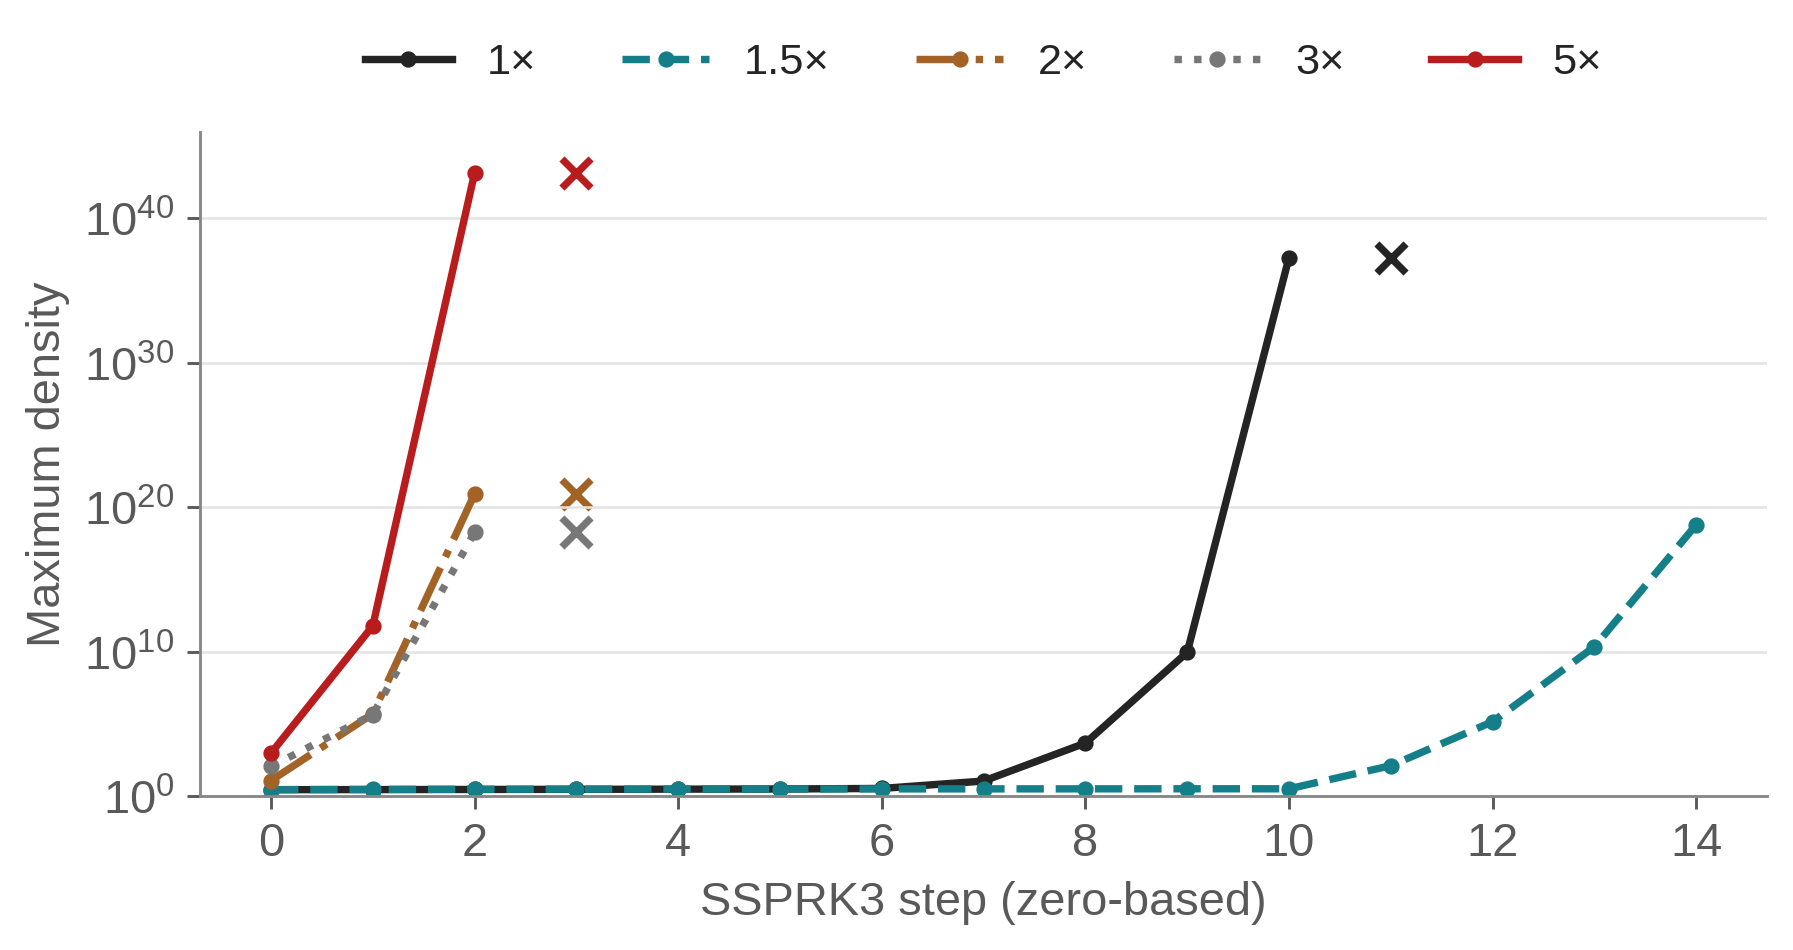
\includegraphics[width=7.115379in,height=3.770000in]{revised_source/assets/art_882e08ef7d9b71.png}};
\node[inner sep=0pt,anchor=center] at ([xshift=10.005417in,yshift=-2.260000in]current page.north west) {\color[HTML]{242424}\fontsize{25.000bp}{30.000bp}\selectfont $\displaystyle F^\pm(U)=\frac12\left(F(U)\pm\alpha U\right)$};
\node[inner sep=0pt,anchor=center] at ([xshift=9.223987in,yshift=-3.155000in]current page.north west) {\color[HTML]{242424}\fontsize{23.232bp}{27.878bp}\selectfont $\displaystyle \mathrm{CFL}_{LF}\sim\frac{\alpha\Delta t}{\Delta x}$};
\node[anchor=north west,inner sep=0pt,outer sep=0pt,text={rgb,255:red,36;green,36;blue,36},align=left,text width=4.500000in,font={\fontsize{15.40bp}{16.63bp}\selectfont \bfseries }] at ([xshift=8.150000in,yshift=-3.730000in]current page.north west) {Fixed Δt confounds the stability scale};
\node[anchor=north west,inner sep=0pt,outer sep=0pt,text={rgb,255:red,89;green,89;blue,89},align=left,text width=4.500000in,font={\fontsize{14.10bp}{15.23bp}\selectfont }] at ([xshift=8.150000in,yshift=-4.070000in]current page.north west) {Neural inputs changed too. Earlier divergence\\ does not show that dissipation itself is harmful.};
\node[anchor=north west,inner sep=0pt,outer sep=0pt,text={rgb,255:red,36;green,36;blue,36},align=left,text width=4.500000in,font={\fontsize{15.40bp}{16.63bp}\selectfont \bfseries }] at ([xshift=8.150000in,yshift=-4.620000in]current page.north west) {Roe conditioning remains a hypothesis};
\node[anchor=north west,inner sep=0pt,outer sep=0pt,text={rgb,255:red,89;green,89;blue,89},align=left,text width=4.500000in,font={\fontsize{14.10bp}{15.23bp}\selectfont }] at ([xshift=8.150000in,yshift=-4.960000in]current page.north west) {No trace establishes it as the initiating cause.};
\node[anchor=north west,inner sep=0pt,outer sep=0pt,text={rgb,255:red,36;green,36;blue,36},align=left,text width=4.500000in,font={\fontsize{15.40bp}{16.63bp}\selectfont \bfseries }] at ([xshift=8.150000in,yshift=-5.510000in]current page.north west) {Next: matched CFL + classical TENO5};
\node[anchor=north west,inner sep=0pt,outer sep=0pt,text={rgb,255:red,89;green,89;blue,89},align=left,text width=4.500000in,font={\fontsize{14.10bp}{15.23bp}\selectfont }] at ([xshift=8.150000in,yshift=-5.850000in]current page.north west) {First-invalid RK stages and cond(R) tracing.};
\node[anchor=north west,inner sep=0pt,outer sep=0pt,text={rgb,255:red,89;green,89;blue,89},align=left,text width=7.100000in,font={\fontsize{12.70bp}{13.72bp}\selectfont }] at ([xshift=0.830000in,yshift=-6.000000in]current page.north west) {×: next non-finite step. 1.5× ends finite but enormous.};
\path[fill={rgb,255:red,36;green,36;blue,36},draw=none] ([xshift=0.600000in,yshift=-6.260000in]current page.north west) rectangle ([xshift=0.642000in,yshift=-6.690000in]current page.north west);
\node[anchor=north west,inner sep=0pt,outer sep=0pt,text={rgb,255:red,36;green,36;blue,36},align=left,text width=11.900000in,font={\fontsize{15.00bp}{16.20bp}\selectfont }] at ([xshift=0.770000in,yshift=-6.250000in]current page.north west) {The experiment was confounded: dissipation, effective timestep restriction,};
\node[anchor=north west,inner sep=0pt,outer sep=0pt,text={rgb,255:red,36;green,36;blue,36},align=left,text width=11.900000in,font={\fontsize{15.00bp}{16.20bp}\selectfont }] at ([xshift=0.770000in,yshift=-6.490000in]current page.north west) {and neural inputs changed simultaneously.};
\node[anchor=north west,inner sep=0pt,outer sep=0pt,text={rgb,255:red,89;green,89;blue,89},align=left,text width=11.950000in,font={\fontsize{8.50bp}{9.18bp}\selectfont }] at ([xshift=0.660000in,yshift=-6.800000in]current page.north west) {Data: models/euler\_instability\_trace.csv. Test: EulerInstability\_TraceCapture.py:66–114. No unique cause established.};
\end{tikzpicture}
\end{frame}
% Slide 6: MAIN
\begin{frame}[plain]
\begin{tikzpicture}[remember picture,overlay]
\node[anchor=north west,inner sep=0pt,outer sep=0pt,text={rgb,255:red,36;green,36;blue,36},align=left,text width=10.900000in,font={\fontsize{10.50bp}{11.34bp}\selectfont \bfseries }] at ([xshift=0.600000in,yshift=-0.300000in]current page.north west) {ATTEMPTED FIX · COMPUTATIONAL SURVIVAL VERSUS PHYSICAL BALANCE};
\node[anchor=north west,inner sep=0pt,outer sep=0pt,text={rgb,255:red,36;green,36;blue,36},align=left,text width=12.050000in,font={\fontsize{27.00bp}{29.16bp}\selectfont \bfseries }] at ([xshift=0.600000in,yshift=-0.780000in]current page.north west) {Direct state repair breaks the conservative budget};
\path[fill={rgb,255:red,222;green,222;blue,222},draw=none] ([xshift=0.600000in,yshift=-1.430000in]current page.north west) rectangle ([xshift=12.700000in,yshift=-1.445000in]current page.north west);
\path[fill={rgb,255:red,222;green,222;blue,222},draw=none] ([xshift=0.600000in,yshift=-7.030000in]current page.north west) rectangle ([xshift=12.700000in,yshift=-7.042000in]current page.north west);
\node[anchor=north west,inner sep=0pt,outer sep=0pt,text={rgb,255:red,89;green,89;blue,89},align=left,text width=7.200000in,font={\fontsize{9.00bp}{9.72bp}\selectfont }] at ([xshift=0.600000in,yshift=-7.150000in]current page.north west) {SHOCKS \& WENO   /   YASSER BAOUZIL};
\node[anchor=north west,inner sep=0pt,outer sep=0pt,text={rgb,255:red,89;green,89;blue,89},align=right,text width=1.100000in,font={\fontsize{10.00bp}{10.80bp}\selectfont }] at ([xshift=11.600000in,yshift=-7.120000in]current page.north west) {06 / 9};
\node[anchor=north west,inner sep=0pt] at ([xshift=9.543659in,yshift=-7.120000in]current page.north west) {
\includegraphics[width=1.312683in,height=0.270000in]{revised_source/assets/art_bf8a20b59a0b57.png}};
\node[inner sep=0pt,anchor=center] at ([xshift=3.223611in,yshift=-2.165000in]current page.north west) {\color[HTML]{242424}\fontsize{25.000bp}{30.000bp}\selectfont $\displaystyle \bar U_i^{n+1}=\bar U_i^n-\frac{\Delta t}{\Delta x}\left(\widehat F_{i+1/2}-\widehat F_{i-1/2}\right)$};
\node[inner sep=0pt,anchor=center] at ([xshift=10.477222in,yshift=-2.175000in]current page.north west) {\color[HTML]{242424}\fontsize{21.000bp}{25.200bp}\selectfont $\displaystyle \Delta M_{\rm repair}=\Delta x\sum_i(\rho_i^{after}-\rho_i^{before})$};
\path[fill={rgb,255:red,245;green,245;blue,245},draw=none,rounded corners=3bp] ([xshift=0.600000in,yshift=-2.910000in]current page.north west) rectangle ([xshift=6.530000in,yshift=-5.190000in]current page.north west);
\node[anchor=north west,inner sep=0pt,outer sep=0pt,text={rgb,255:red,36;green,36;blue,36},align=left,text width=5.490000in,font={\fontsize{17.70bp}{19.12bp}\selectfont \bfseries }] at ([xshift=0.820000in,yshift=-3.100000in]current page.north west) {Implemented · post-update repair};
\path[fill={rgb,255:red,245;green,245;blue,245},draw=none,rounded corners=3bp] ([xshift=6.790000in,yshift=-2.910000in]current page.north west) rectangle ([xshift=12.720000in,yshift=-5.190000in]current page.north west);
\node[anchor=north west,inner sep=0pt,outer sep=0pt,text={rgb,255:red,36;green,36;blue,36},align=left,text width=5.490000in,font={\fontsize{17.70bp}{19.12bp}\selectfont \bfseries }] at ([xshift=7.010000in,yshift=-3.100000in]current page.north west) {Established · flux limiting (not tested)};
\path[fill={rgb,255:red,255;green,255;blue,255},draw={rgb,255:red,222;green,222;blue,222}] ([xshift=0.850000in,yshift=-3.760000in]current page.north west) rectangle ([xshift=2.360000in,yshift=-4.320000in]current page.north west);
\node[anchor=north west,inner sep=0pt,outer sep=0pt,text={rgb,255:red,36;green,36;blue,36},align=center,text width=1.390000in,font={\fontsize{13.80bp}{14.90bp}\selectfont }] at ([xshift=0.910000in,yshift=-3.910000in]current page.north west) {Flux update};
\node[anchor=north west,inner sep=0pt,outer sep=0pt,text={rgb,255:red,89;green,89;blue,89},align=center,text width=0.300000in,font={\fontsize{20.52bp}{22.16bp}\selectfont }] at ([xshift=2.370000in,yshift=-3.880000in]current page.north west) {→};
\path[fill={rgb,255:red,255;green,255;blue,255},draw={rgb,255:red,222;green,222;blue,222}] ([xshift=2.690000in,yshift=-3.760000in]current page.north west) rectangle ([xshift=4.200000in,yshift=-4.320000in]current page.north west);
\node[anchor=north west,inner sep=0pt,outer sep=0pt,text={rgb,255:red,36;green,36;blue,36},align=center,text width=1.390000in,font={\fontsize{13.80bp}{14.90bp}\selectfont }] at ([xshift=2.750000in,yshift=-3.910000in]current page.north west) {Invalid stage};
\node[anchor=north west,inner sep=0pt,outer sep=0pt,text={rgb,255:red,89;green,89;blue,89},align=center,text width=0.300000in,font={\fontsize{20.52bp}{22.16bp}\selectfont }] at ([xshift=4.210000in,yshift=-3.880000in]current page.north west) {→};
\path[fill={rgb,255:red,255;green,255;blue,255},draw={rgb,255:red,222;green,222;blue,222}] ([xshift=4.530000in,yshift=-3.760000in]current page.north west) rectangle ([xshift=6.040000in,yshift=-4.320000in]current page.north west);
\node[anchor=north west,inner sep=0pt,outer sep=0pt,text={rgb,255:red,36;green,36;blue,36},align=center,text width=1.390000in,font={\fontsize{13.80bp}{14.90bp}\selectfont }] at ([xshift=4.590000in,yshift=-3.910000in]current page.north west) {Overwrite cell};
\path[fill={rgb,255:red,255;green,255;blue,255},draw={rgb,255:red,222;green,222;blue,222}] ([xshift=7.040000in,yshift=-3.760000in]current page.north west) rectangle ([xshift=8.550000in,yshift=-4.320000in]current page.north west);
\node[anchor=north west,inner sep=0pt,outer sep=0pt,text={rgb,255:red,36;green,36;blue,36},align=center,text width=1.390000in,font={\fontsize{13.80bp}{14.90bp}\selectfont }] at ([xshift=7.100000in,yshift=-3.910000in]current page.north west) {NN flux};
\node[anchor=north west,inner sep=0pt,outer sep=0pt,text={rgb,255:red,89;green,89;blue,89},align=center,text width=0.300000in,font={\fontsize{20.52bp}{22.16bp}\selectfont }] at ([xshift=8.560000in,yshift=-3.880000in]current page.north west) {→};
\path[fill={rgb,255:red,255;green,255;blue,255},draw={rgb,255:red,222;green,222;blue,222}] ([xshift=8.880000in,yshift=-3.760000in]current page.north west) rectangle ([xshift=10.390000in,yshift=-4.320000in]current page.north west);
\node[anchor=north west,inner sep=0pt,outer sep=0pt,text={rgb,255:red,36;green,36;blue,36},align=center,text width=1.390000in,font={\fontsize{13.80bp}{14.90bp}\selectfont }] at ([xshift=8.940000in,yshift=-3.910000in]current page.north west) {Limit face flux};
\node[anchor=north west,inner sep=0pt,outer sep=0pt,text={rgb,255:red,89;green,89;blue,89},align=center,text width=0.300000in,font={\fontsize{20.52bp}{22.16bp}\selectfont }] at ([xshift=10.400000in,yshift=-3.880000in]current page.north west) {→};
\path[fill={rgb,255:red,255;green,255;blue,255},draw={rgb,255:red,222;green,222;blue,222}] ([xshift=10.720000in,yshift=-3.760000in]current page.north west) rectangle ([xshift=12.230000in,yshift=-4.320000in]current page.north west);
\node[anchor=north west,inner sep=0pt,outer sep=0pt,text={rgb,255:red,36;green,36;blue,36},align=center,text width=1.390000in,font={\fontsize{13.80bp}{14.90bp}\selectfont }] at ([xshift=10.780000in,yshift=-3.910000in]current page.north west) {Update cells};
\node[anchor=north west,inner sep=0pt,outer sep=0pt,text={rgb,255:red,36;green,36;blue,36},align=left,text width=5.240000in,font={\fontsize{14.60bp}{15.77bp}\selectfont \bfseries }] at ([xshift=0.900000in,yshift=-4.500000in]current page.north west) {One repaired stage · final RK-weighted source};
\node[anchor=north west,inner sep=0pt,outer sep=0pt,text={rgb,255:red,185;green,28;blue,28},align=left,text width=5.240000in,font={\fontsize{15.50bp}{16.74bp}\selectfont }] at ([xshift=0.900000in,yshift=-4.860000in]current page.north west) {Δmass ≈ +0.001611 · Δenergy ≈ +0.000889};
\node[anchor=north west,inner sep=0pt,outer sep=0pt,text={rgb,255:red,89;green,89;blue,89},align=left,text width=5.330000in,font={\fontsize{15.50bp}{18.29bp}\selectfont }] at ([xshift=7.050000in,yshift=-4.530000in]current page.north west) {Shared face flux preserves the discrete budget.\\ Needs an admissible baseline, factors and CFL.};
\node[anchor=north west,inner sep=0pt,outer sep=0pt,text={rgb,255:red,89;green,89;blue,89},align=left,text width=6.010000in,font={\fontsize{17.00bp}{22.10bp}\selectfont }] at ([xshift=0.760000in,yshift=-5.550000in]current page.north west) {Post-repair penalties once hid violations.\\ Guarded training ≠ unguarded validation.};
\node[anchor=north west,inner sep=0pt,outer sep=0pt,text={rgb,255:red,89;green,89;blue,89},align=left,text width=5.420000in,font={\fontsize{17.00bp}{22.10bp}\selectfont }] at ([xshift=7.030000in,yshift=-5.550000in]current page.north west) {Not implemented or validated\\ in this neural solver.};
\path[fill={rgb,255:red,36;green,36;blue,36},draw=none] ([xshift=0.600000in,yshift=-6.390000in]current page.north west) rectangle ([xshift=0.642000in,yshift=-6.740000in]current page.north west);
\node[anchor=north west,inner sep=0pt,outer sep=0pt,text={rgb,255:red,36;green,36;blue,36},align=left,text width=11.900000in,font={\fontsize{17.00bp}{18.36bp}\selectfont }] at ([xshift=0.770000in,yshift=-6.380000in]current page.north west) {A finite repaired trajectory does not certify the unguarded learned solver.};
\node[anchor=north west,inner sep=0pt,outer sep=0pt,text={rgb,255:red,89;green,89;blue,89},align=left,text width=11.950000in,font={\fontsize{8.50bp}{9.18bp}\selectfont }] at ([xshift=0.660000in,yshift=-6.800000in]current page.north west) {Measured: results/repair/repair.json, soft/.75, one repaired stage row. Conservative remedy: Hu–Adams–Shu (2013).};
\end{tikzpicture}
\end{frame}
% Slide 7: MAIN
\begin{frame}[plain]
\begin{tikzpicture}[remember picture,overlay]
\node[anchor=north west,inner sep=0pt,outer sep=0pt,text={rgb,255:red,36;green,36;blue,36},align=left,text width=10.900000in,font={\fontsize{10.50bp}{11.34bp}\selectfont \bfseries }] at ([xshift=0.600000in,yshift=-0.300000in]current page.north west) {LATER V2 · FROZEN MODEL AND SELECTED SOFT STRENGTH .25};
\node[anchor=north west,inner sep=0pt,outer sep=0pt,text={rgb,255:red,36;green,36;blue,36},align=left,text width=12.050000in,font={\fontsize{27.00bp}{29.16bp}\selectfont \bfseries }] at ([xshift=0.600000in,yshift=-0.780000in]current page.north west) {Validation gains did not imply universal transfer};
\path[fill={rgb,255:red,222;green,222;blue,222},draw=none] ([xshift=0.600000in,yshift=-1.430000in]current page.north west) rectangle ([xshift=12.700000in,yshift=-1.445000in]current page.north west);
\path[fill={rgb,255:red,222;green,222;blue,222},draw=none] ([xshift=0.600000in,yshift=-7.030000in]current page.north west) rectangle ([xshift=12.700000in,yshift=-7.042000in]current page.north west);
\node[anchor=north west,inner sep=0pt,outer sep=0pt,text={rgb,255:red,89;green,89;blue,89},align=left,text width=7.200000in,font={\fontsize{9.00bp}{9.72bp}\selectfont }] at ([xshift=0.600000in,yshift=-7.150000in]current page.north west) {SHOCKS \& WENO   /   YASSER BAOUZIL};
\node[anchor=north west,inner sep=0pt,outer sep=0pt,text={rgb,255:red,89;green,89;blue,89},align=right,text width=1.100000in,font={\fontsize{10.00bp}{10.80bp}\selectfont }] at ([xshift=11.600000in,yshift=-7.120000in]current page.north west) {07 / 9};
\node[anchor=north west,inner sep=0pt] at ([xshift=9.543659in,yshift=-7.120000in]current page.north west) {
\includegraphics[width=1.312683in,height=0.270000in]{revised_source/assets/art_bf8a20b59a0b57.png}};
\node[anchor=north west,inner sep=0pt] at ([xshift=0.550000in,yshift=-1.930905in]current page.north west) {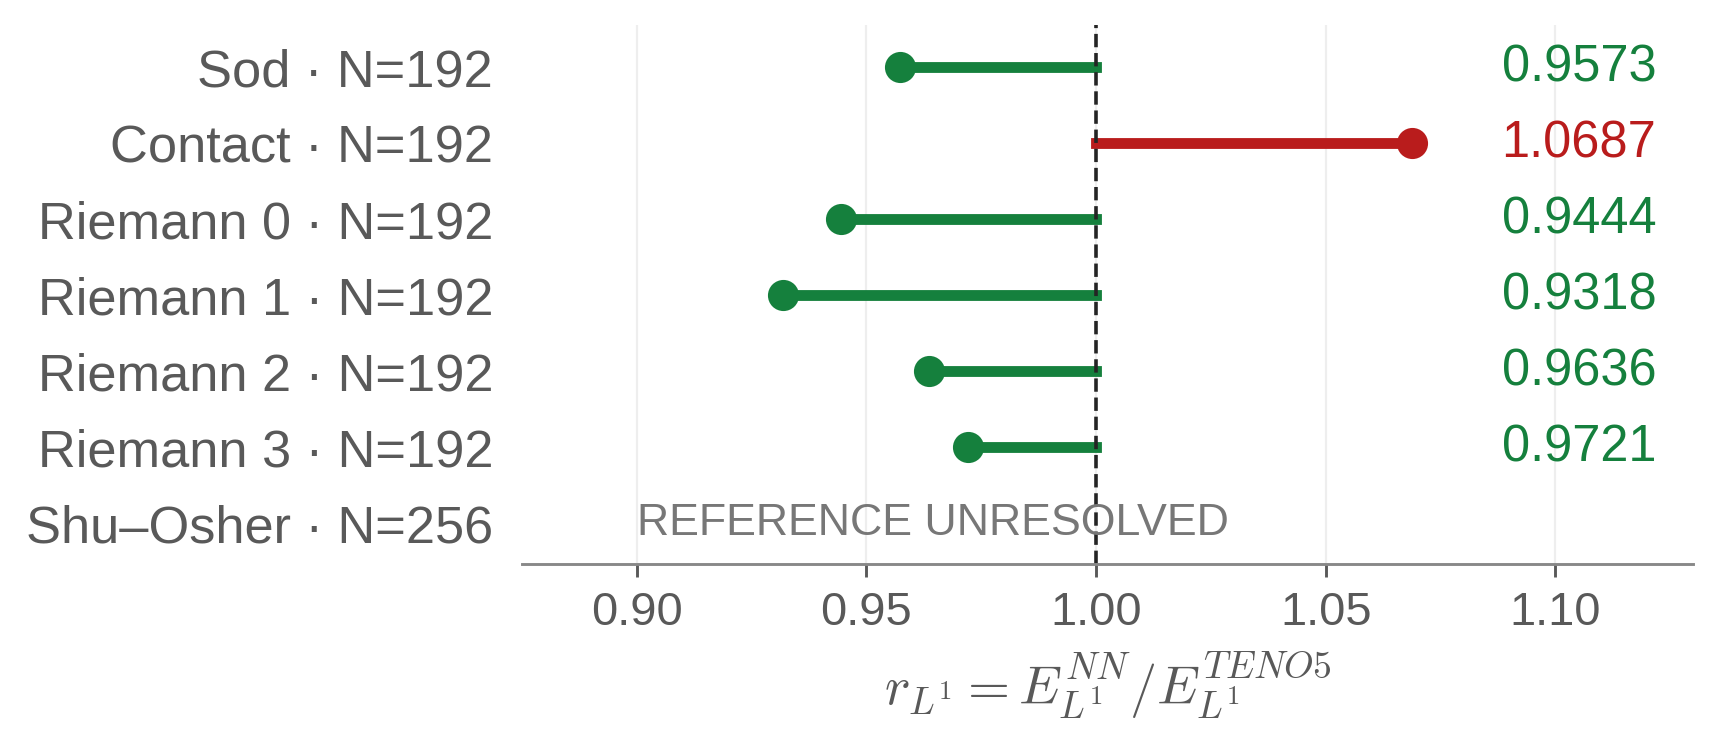
\includegraphics[width=7.070000in,height=3.068191in]{revised_source/assets/art_f3e71576ce15ed.png}};
\node[anchor=north west,inner sep=0pt,outer sep=0pt,text={rgb,255:red,21;green,128;blue,61},align=left,text width=4.630000in,font={\fontsize{34.00bp}{36.72bp}\selectfont \bfseries }] at ([xshift=7.930000in,yshift=-1.830000in]current page.north west) {0.94794};
\node[anchor=north west,inner sep=0pt,outer sep=0pt,text={rgb,255:red,89;green,89;blue,89},align=left,text width=4.670000in,font={\fontsize{16.80bp}{21.50bp}\selectfont }] at ([xshift=7.960000in,yshift=-2.530000in]current page.north west) {Validation macro L\textsuperscript{1} ratio\\ 307 short Euler IVPs · no invalid stages};
\node[anchor=north west,inner sep=0pt] at ([xshift=7.894683in,yshift=-3.360000in]current page.north west) {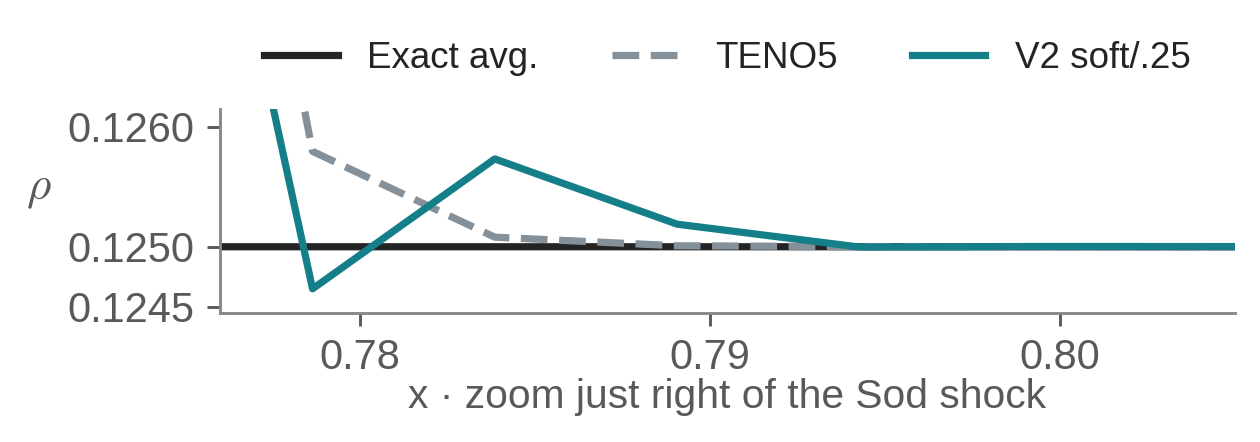
\includegraphics[width=4.760633in,height=1.670000in]{revised_source/assets/art_ca6ef537d4e26b.png}};
\node[anchor=north west,inner sep=0pt,outer sep=0pt,text={rgb,255:red,89;green,89;blue,89},align=left,text width=4.610000in,font={\fontsize{15.70bp}{18.84bp}\selectfont }] at ([xshift=7.980000in,yshift=-5.060000in]current page.north west) {Sod N=192: 4.3\% lower L\textsuperscript{1}, but TV rises\\ and density undershoot ≈ 3.51×10\textsuperscript{-4}.};
\path[fill={rgb,255:red,245;green,245;blue,245},draw=none,rounded corners=3bp] ([xshift=0.650000in,yshift=-5.280000in]current page.north west) rectangle ([xshift=7.610000in,yshift=-6.380000in]current page.north west);
\node[anchor=north west,inner sep=0pt,outer sep=0pt,text={rgb,255:red,36;green,36;blue,36},align=left,text width=6.560000in,font={\fontsize{17.30bp}{18.68bp}\selectfont \bfseries }] at ([xshift=0.860000in,yshift=-5.420000in]current page.north west) {Woodward–Colella blast · N=128, 256};
\node[anchor=north west,inner sep=0pt,outer sep=0pt,text={rgb,255:red,185;green,28;blue,28},align=left,text width=6.560000in,font={\fontsize{21.00bp}{22.68bp}\selectfont \bfseries }] at ([xshift=0.860000in,yshift=-5.780000in]current page.north west) {FAILED — no accuracy score};
\node[anchor=north west,inner sep=0pt,outer sep=0pt,text={rgb,255:red,89;green,89;blue,89},align=left,text width=6.560000in,font={\fontsize{13.80bp}{14.90bp}\selectfont }] at ([xshift=0.860000in,yshift=-6.120000in]current page.north west) {V2 non-finite; classical TENO5 completed both.};
\node[anchor=north west,inner sep=0pt,outer sep=0pt,text={rgb,255:red,36;green,36;blue,36},align=left,text width=4.690000in,font={\fontsize{13.90bp}{15.01bp}\selectfont \bfseries }] at ([xshift=7.980000in,yshift=-5.750000in]current page.north west) {Possible contributors · not isolated causes};
\node[anchor=north west,inner sep=0pt,outer sep=0pt,text={rgb,255:red,89;green,89;blue,89},align=left,text width=4.690000in,font={\fontsize{13.60bp}{15.64bp}\selectfont }] at ([xshift=7.980000in,yshift=-6.030000in]current page.north west) {Shock strength, interactions, reflective walls.\\ State feedback; training / deployment mismatch.};
\path[fill={rgb,255:red,36;green,36;blue,36},draw=none] ([xshift=0.600000in,yshift=-6.490000in]current page.north west) rectangle ([xshift=0.642000in,yshift=-6.730000in]current page.north west);
\node[anchor=north west,inner sep=0pt,outer sep=0pt,text={rgb,255:red,36;green,36;blue,36},align=left,text width=11.900000in,font={\fontsize{15.60bp}{16.85bp}\selectfont }] at ([xshift=0.770000in,yshift=-6.480000in]current page.north west) {Short-horizon validation did not guarantee stability under stronger out-of-distribution Euler dynamics.};
\node[anchor=north west,inner sep=0pt,outer sep=0pt,text={rgb,255:red,89;green,89;blue,89},align=left,text width=11.950000in,font={\fontsize{8.50bp}{9.18bp}\selectfont }] at ([xshift=0.660000in,yshift=-6.800000in]current page.north west) {Frozen V2 only. Data: full-validation/summary.json · independent/benchmark.json · wall-closure/benchmark.json.};
\end{tikzpicture}
\end{frame}
% Slide 8: MAIN
\begin{frame}[plain]
\begin{tikzpicture}[remember picture,overlay]
\node[anchor=north west,inner sep=0pt,outer sep=0pt,text={rgb,255:red,36;green,36;blue,36},align=left,text width=10.900000in,font={\fontsize{10.50bp}{11.34bp}\selectfont \bfseries }] at ([xshift=0.600000in,yshift=-0.300000in]current page.north west) {CONSISTENCY INVESTIGATION · GENERAL NONLINEAR SMOOTH EULER DATA};
\node[anchor=north west,inner sep=0pt,outer sep=0pt,text={rgb,255:red,36;green,36;blue,36},align=left,text width=12.050000in,font={\fontsize{27.00bp}{29.16bp}\selectfont \bfseries }] at ([xshift=0.600000in,yshift=-0.780000in]current page.north west) {The classical FV pipeline also limited accuracy};
\path[fill={rgb,255:red,222;green,222;blue,222},draw=none] ([xshift=0.600000in,yshift=-1.430000in]current page.north west) rectangle ([xshift=12.700000in,yshift=-1.445000in]current page.north west);
\path[fill={rgb,255:red,222;green,222;blue,222},draw=none] ([xshift=0.600000in,yshift=-7.030000in]current page.north west) rectangle ([xshift=12.700000in,yshift=-7.042000in]current page.north west);
\node[anchor=north west,inner sep=0pt,outer sep=0pt,text={rgb,255:red,89;green,89;blue,89},align=left,text width=7.200000in,font={\fontsize{9.00bp}{9.72bp}\selectfont }] at ([xshift=0.600000in,yshift=-7.150000in]current page.north west) {SHOCKS \& WENO   /   YASSER BAOUZIL};
\node[anchor=north west,inner sep=0pt,outer sep=0pt,text={rgb,255:red,89;green,89;blue,89},align=right,text width=1.100000in,font={\fontsize{10.00bp}{10.80bp}\selectfont }] at ([xshift=11.600000in,yshift=-7.120000in]current page.north west) {08 / 9};
\node[anchor=north west,inner sep=0pt] at ([xshift=9.543659in,yshift=-7.120000in]current page.north west) {
\includegraphics[width=1.312683in,height=0.270000in]{revised_source/assets/art_bf8a20b59a0b57.png}};
\node[anchor=north west,inner sep=0pt] at ([xshift=0.600000in,yshift=-1.918921in]current page.north west) {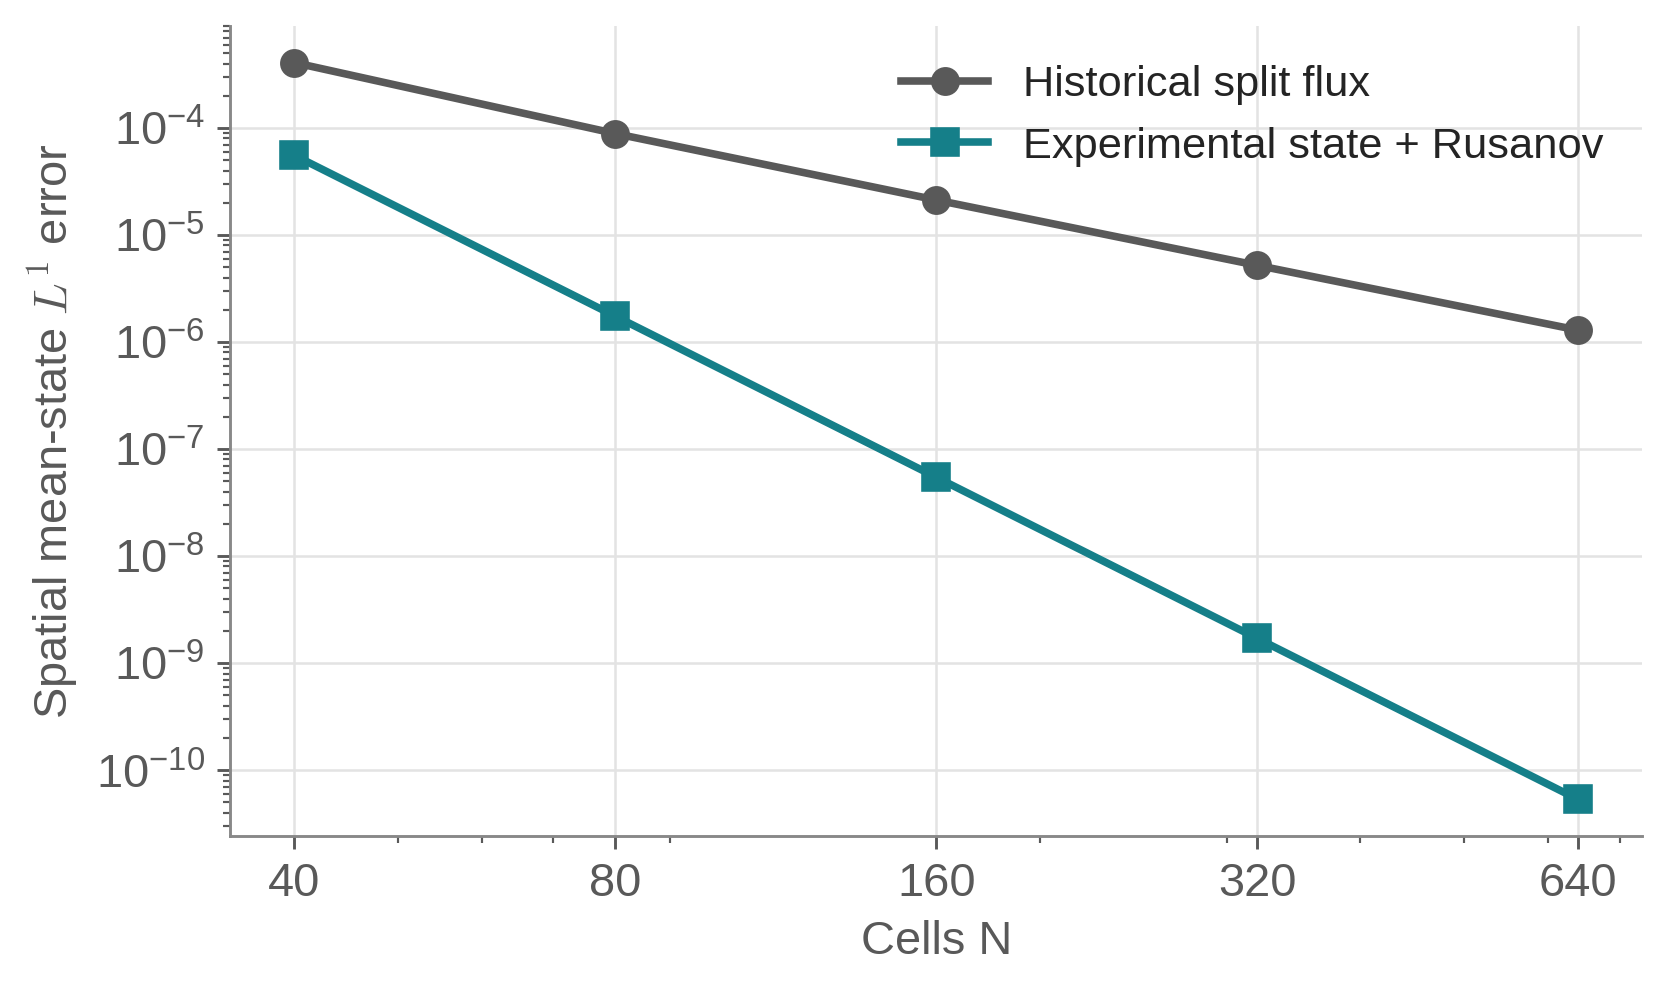
\includegraphics[width=7.080000in,height=4.202158in]{revised_source/assets/art_9460c9cc254a0c.png}};
\node[inner sep=0pt,anchor=center] at ([xshift=9.297292in,yshift=-2.285000in]current page.north west) {\color[HTML]{242424}\fontsize{30.000bp}{36.000bp}\selectfont $\displaystyle \overline{F(U)}\ne F(\bar U)$};
\node[anchor=north west,inner sep=0pt,outer sep=0pt,text={rgb,255:red,89;green,89;blue,89},align=left,text width=4.600000in,font={\fontsize{18.00bp}{22.50bp}\selectfont }] at ([xshift=8.020000in,yshift=-2.940000in]current page.north west) {Nonlinear flux evaluation and\\ cell averaging do not commute.};
\node[anchor=north west,inner sep=0pt,outer sep=0pt,text={rgb,255:red,36;green,36;blue,36},align=left,text width=4.590000in,font={\fontsize{19.00bp}{24.32bp}\selectfont \bfseries }] at ([xshift=8.020000in,yshift=-3.930000in]current page.north west) {Historical FV path: order ≈ 2.01\\ State + Rusanov: order ≈ 5.00};
\node[anchor=north west,inner sep=0pt,outer sep=0pt,text={rgb,255:red,89;green,89;blue,89},align=left,text width=4.640000in,font={\fontsize{16.50bp}{20.46bp}\selectfont }] at ([xshift=8.020000in,yshift=-5.070000in]current page.north west) {Experimental remedy\\ Consistent FV state reconstruction.\\ Shock/positivity behavior unvalidated.};
\path[fill={rgb,255:red,36;green,36;blue,36},draw=none] ([xshift=0.600000in,yshift=-6.350000in]current page.north west) rectangle ([xshift=0.642000in,yshift=-6.700000in]current page.north west);
\node[anchor=north west,inner sep=0pt,outer sep=0pt,text={rgb,255:red,36;green,36;blue,36},align=left,text width=11.900000in,font={\fontsize{17.00bp}{18.36bp}\selectfont }] at ([xshift=0.770000in,yshift=-6.340000in]current page.north west) {This limitation affects classical TENO5 too; it is not a neural-only failure.};
\node[anchor=north west,inner sep=0pt,outer sep=0pt,text={rgb,255:red,89;green,89;blue,89},align=left,text width=11.950000in,font={\fontsize{8.50bp}{9.18bp}\selectfont }] at ([xshift=0.660000in,yshift=-6.800000in]current page.north west) {Data: nonlinear\_euler.json; semidiscrete exact-average divergence. WENO7 details → Backup B. Wall correction ≠ blast robustness.};
\end{tikzpicture}
\end{frame}
% Slide 9: MAIN
\begin{frame}[plain]
\begin{tikzpicture}[remember picture,overlay]
\node[anchor=north west,inner sep=0pt,outer sep=0pt,text={rgb,255:red,36;green,36;blue,36},align=left,text width=10.900000in,font={\fontsize{10.50bp}{11.34bp}\selectfont \bfseries }] at ([xshift=0.600000in,yshift=-0.300000in]current page.north west) {RESEARCH DIRECTION · RELIABLE MACHINE-LEARNING-ASSISTED METHODS};
\node[anchor=north west,inner sep=0pt,outer sep=0pt,text={rgb,255:red,36;green,36;blue,36},align=left,text width=12.050000in,font={\fontsize{27.00bp}{29.16bp}\selectfont \bfseries }] at ([xshift=0.600000in,yshift=-0.780000in]current page.north west) {Learn within verifiable numerical constraints};
\path[fill={rgb,255:red,222;green,222;blue,222},draw=none] ([xshift=0.600000in,yshift=-1.430000in]current page.north west) rectangle ([xshift=12.700000in,yshift=-1.445000in]current page.north west);
\path[fill={rgb,255:red,222;green,222;blue,222},draw=none] ([xshift=0.600000in,yshift=-7.030000in]current page.north west) rectangle ([xshift=12.700000in,yshift=-7.042000in]current page.north west);
\node[anchor=north west,inner sep=0pt,outer sep=0pt,text={rgb,255:red,89;green,89;blue,89},align=left,text width=7.200000in,font={\fontsize{9.00bp}{9.72bp}\selectfont }] at ([xshift=0.600000in,yshift=-7.150000in]current page.north west) {SHOCKS \& WENO   /   YASSER BAOUZIL};
\node[anchor=north west,inner sep=0pt,outer sep=0pt,text={rgb,255:red,89;green,89;blue,89},align=right,text width=1.100000in,font={\fontsize{10.00bp}{10.80bp}\selectfont }] at ([xshift=11.600000in,yshift=-7.120000in]current page.north west) {09 / 9};
\node[anchor=north west,inner sep=0pt] at ([xshift=9.543659in,yshift=-7.120000in]current page.north west) {
\includegraphics[width=1.312683in,height=0.270000in]{revised_source/assets/art_bf8a20b59a0b57.png}};
\path[fill={rgb,255:red,245;green,245;blue,245},draw=none,rounded corners=3bp] ([xshift=0.600000in,yshift=-1.760000in]current page.north west) rectangle ([xshift=4.460000in,yshift=-2.990000in]current page.north west);
\node[anchor=north west,inner sep=0pt,outer sep=0pt,text={rgb,255:red,36;green,36;blue,36},align=left,text width=3.480000in,font={\fontsize{18.00bp}{19.44bp}\selectfont \bfseries }] at ([xshift=0.790000in,yshift=-1.940000in]current page.north west) {Observed limitations};
\node[anchor=north west,inner sep=0pt,outer sep=0pt,text={rgb,255:red,89;green,89;blue,89},align=left,text width=3.480000in,font={\fontsize{14.40bp}{17.28bp}\selectfont }] at ([xshift=0.790000in,yshift=-2.390000in]current page.north west) {Negative stages · repair sources\\ Transfer gaps · accuracy/oscillations};
\path[fill={rgb,255:red,245;green,245;blue,245},draw=none,rounded corners=3bp] ([xshift=4.730000in,yshift=-1.760000in]current page.north west) rectangle ([xshift=8.590000in,yshift=-2.990000in]current page.north west);
\node[anchor=north west,inner sep=0pt,outer sep=0pt,text={rgb,255:red,36;green,36;blue,36},align=left,text width=3.480000in,font={\fontsize{18.00bp}{19.44bp}\selectfont \bfseries }] at ([xshift=4.920000in,yshift=-1.940000in]current page.north west) {Established techniques};
\node[anchor=north west,inner sep=0pt,outer sep=0pt,text={rgb,255:red,89;green,89;blue,89},align=left,text width=3.480000in,font={\fontsize{14.40bp}{17.28bp}\selectfont }] at ([xshift=4.920000in,yshift=-2.390000in]current page.north west) {Flux limiting · invariant domains\\ Moments · conditional SSP};
\path[fill={rgb,255:red,245;green,245;blue,245},draw=none,rounded corners=3bp] ([xshift=8.860000in,yshift=-1.760000in]current page.north west) rectangle ([xshift=12.720000in,yshift=-2.990000in]current page.north west);
\node[anchor=north west,inner sep=0pt,outer sep=0pt,text={rgb,255:red,36;green,36;blue,36},align=left,text width=3.480000in,font={\fontsize{18.00bp}{19.44bp}\selectfont \bfseries }] at ([xshift=9.050000in,yshift=-1.940000in]current page.north west) {Open research};
\node[anchor=north west,inner sep=0pt,outer sep=0pt,text={rgb,255:red,89;green,89;blue,89},align=left,text width=3.480000in,font={\fontsize{14.40bp}{17.28bp}\selectfont }] at ([xshift=9.050000in,yshift=-2.390000in]current page.north west) {Admissible learned corrections\\ DG/SIAC moments · residual checks};
\node[anchor=north west,inner sep=0pt,outer sep=0pt,text={rgb,255:red,36;green,36;blue,36},align=left,text width=6.550000in,font={\fontsize{18.00bp}{19.44bp}\selectfont \bfseries }] at ([xshift=0.780000in,yshift=-3.190000in]current page.north west) {Shared-face limited flux};
\node[inner sep=0pt,anchor=center] at ([xshift=3.410764in,yshift=-4.050000in]current page.north west) {\color[HTML]{242424}\fontsize{27.000bp}{32.400bp}\selectfont $\displaystyle \widehat F^{limited}=\widehat F^{LO}+\theta\left(\widehat F^{NN}-\widehat F^{LO}\right)$};
\node[anchor=north west,inner sep=0pt,outer sep=0pt,text={rgb,255:red,36;green,36;blue,36},align=left,text width=4.560000in,font={\fontsize{18.00bp}{19.44bp}\selectfont \bfseries }] at ([xshift=8.040000in,yshift=-3.190000in]current page.north west) {Independent space–time residual};
\node[inner sep=0pt,anchor=center] at ([xshift=9.618681in,yshift=-4.050000in]current page.north west) {\color[HTML]{242424}\fontsize{27.000bp}{32.400bp}\selectfont $\displaystyle \mathscr R=\partial_t\widehat U+\partial_xF(\widehat U)$};
\node[anchor=north west,inner sep=0pt,outer sep=0pt,text={rgb,255:red,89;green,89;blue,89},align=left,text width=11.800000in,font={\fontsize{15.00bp}{16.20bp}\selectfont }] at ([xshift=0.790000in,yshift=-4.620000in]current page.north west) {θ in [0,1] alone does not ensure positivity. A residual alone does not certify an error bound.};
\node[anchor=north west,inner sep=0pt,outer sep=0pt,text={rgb,255:red,36;green,36;blue,36},align=left,text width=11.850000in,font={\fontsize{18.00bp}{19.44bp}\selectfont \bfseries }] at ([xshift=0.790000in,yshift=-5.100000in]current page.north west) {Giesselmann, Kwon \& Krumscheid (2026) · RKDG + SIAC};
\node[anchor=north west,inner sep=0pt,outer sep=0pt,text={rgb,255:red,89;green,89;blue,89},align=left,text width=11.850000in,font={\fontsize{15.20bp}{17.63bp}\selectfont }] at ([xshift=0.790000in,yshift=-5.550000in]current page.north west) {Begin with checkable smooth-state, moment and stability assumptions; then test near shocks.\\ The convection–diffusion RKDG–SIAC paper does not certify this neural Euler solver.};
\path[fill={rgb,255:red,36;green,36;blue,36},draw=none] ([xshift=0.600000in,yshift=-6.180000in]current page.north west) rectangle ([xshift=0.642000in,yshift=-6.530000in]current page.north west);
\node[anchor=north west,inner sep=0pt,outer sep=0pt,text={rgb,255:red,36;green,36;blue,36},align=left,text width=11.900000in,font={\fontsize{17.20bp}{18.58bp}\selectfont }] at ([xshift=0.770000in,yshift=-6.170000in]current page.north west) {Can learned high-order reconstruction improve numerical accuracy while retaining\\ provable structural constraints and independently verifiable error control?};
\node[anchor=north west,inner sep=0pt,outer sep=0pt,text={rgb,255:red,89;green,89;blue,89},align=left,text width=11.950000in,font={\fontsize{8.50bp}{9.18bp}\selectfont }] at ([xshift=0.660000in,yshift=-6.800000in]current page.north west) {Hu–Adams–Shu (2013) · Guermond et al. (2018) · Gottlieb et al. (2001) · arXiv:2604.01200. Discussion; backups follow.};
\end{tikzpicture}
\end{frame}
% Slide 10: BACKUP
\begin{frame}[plain]
\begin{tikzpicture}[remember picture,overlay]
\node[anchor=north west,inner sep=0pt,outer sep=0pt,text={rgb,255:red,36;green,36;blue,36},align=left,text width=10.900000in,font={\fontsize{10.50bp}{11.34bp}\selectfont \bfseries }] at ([xshift=0.600000in,yshift=-0.300000in]current page.north west) {BACKUP A · MATHEMATICAL FORMULATION};
\node[anchor=north west,inner sep=0pt,outer sep=0pt,text={rgb,255:red,36;green,36;blue,36},align=left,text width=12.050000in,font={\fontsize{27.00bp}{29.16bp}\selectfont \bfseries }] at ([xshift=0.600000in,yshift=-0.780000in]current page.north west) {Euler reconstruction and SSPRK3: the full map};
\path[fill={rgb,255:red,222;green,222;blue,222},draw=none] ([xshift=0.600000in,yshift=-1.430000in]current page.north west) rectangle ([xshift=12.700000in,yshift=-1.445000in]current page.north west);
\path[fill={rgb,255:red,222;green,222;blue,222},draw=none] ([xshift=0.600000in,yshift=-7.030000in]current page.north west) rectangle ([xshift=12.700000in,yshift=-7.042000in]current page.north west);
\node[anchor=north west,inner sep=0pt,outer sep=0pt,text={rgb,255:red,89;green,89;blue,89},align=left,text width=7.200000in,font={\fontsize{9.00bp}{9.72bp}\selectfont }] at ([xshift=0.600000in,yshift=-7.150000in]current page.north west) {SHOCKS \& WENO   /   YASSER BAOUZIL};
\node[anchor=north west,inner sep=0pt,outer sep=0pt,text={rgb,255:red,89;green,89;blue,89},align=right,text width=2.050000in,font={\fontsize{10.00bp}{10.80bp}\selectfont }] at ([xshift=10.650000in,yshift=-7.120000in]current page.north west) {BACKUP A / 03};
\node[anchor=north west,inner sep=0pt] at ([xshift=9.543659in,yshift=-7.120000in]current page.north west) {
\includegraphics[width=1.312683in,height=0.270000in]{revised_source/assets/art_bf8a20b59a0b57.png}};
\node[anchor=north west,inner sep=0pt,outer sep=0pt,text={rgb,255:red,36;green,36;blue,36},align=left,text width=6.000000in,font={\fontsize{20.00bp}{21.60bp}\selectfont \bfseries }] at ([xshift=0.780000in,yshift=-1.790000in]current page.north west) {Face characteristic decomposition};
\node[inner sep=0pt,anchor=center] at ([xshift=3.362500in,yshift=-2.640000in]current page.north west) {\color[HTML]{242424}\fontsize{24.000bp}{28.800bp}\selectfont $\displaystyle \lambda_j=v-c,\ v,\ v+c,\qquad c=\sqrt{\gamma p/\rho}$};
\node[inner sep=0pt,anchor=center] at ([xshift=3.325139in,yshift=-3.600000in]current page.north west) {\color[HTML]{242424}\fontsize{24.000bp}{28.800bp}\selectfont $\displaystyle g^\pm_{i+1/2,k}=\tfrac12 L_{i+1/2}\left(F(U_k)\pm a_{i+1/2}U_k\right)$};
\node[inner sep=0pt,anchor=center] at ([xshift=3.053681in,yshift=-4.670000in]current page.north west) {\color[HTML]{242424}\fontsize{24.000bp}{28.800bp}\selectfont $\displaystyle \widehat F_{i+1/2}=R_{i+1/2}\left[\mathcal R(g^+)+\mathcal R(g^-)\right]$};
\node[anchor=north west,inner sep=0pt,outer sep=0pt,text={rgb,255:red,89;green,89;blue,89},align=left,text width=6.050000in,font={\fontsize{16.10bp}{20.61bp}\selectfont }] at ([xshift=0.790000in,yshift=-5.470000in]current page.north west) {Same face basis for both LF directions.\\ Negative branch: shift by one cell and reverse.\\ Default a: maximum speed of adjacent cells.};
\node[anchor=north west,inner sep=0pt,outer sep=0pt,text={rgb,255:red,36;green,36;blue,36},align=left,text width=5.300000in,font={\fontsize{19.00bp}{20.52bp}\selectfont \bfseries }] at ([xshift=7.290000in,yshift=-1.790000in]current page.north west) {SSPRK3 · admissible at every stage};
\node[inner sep=0pt,anchor=center] at ([xshift=8.986111in,yshift=-2.740000in]current page.north west) {\color[HTML]{242424}\fontsize{25.000bp}{30.000bp}\selectfont $\displaystyle U^{(1)}=U^n-\Delta tD(U^n)$};
\node[inner sep=0pt,anchor=center] at ([xshift=9.697014in,yshift=-3.795000in]current page.north west) {\color[HTML]{242424}\fontsize{24.000bp}{28.800bp}\selectfont $\displaystyle U^{(2)}=\tfrac34U^n+\tfrac14\left[U^{(1)}-\Delta tD(U^{(1)})\right]$};
\node[inner sep=0pt,anchor=center] at ([xshift=9.766319in,yshift=-4.835000in]current page.north west) {\color[HTML]{242424}\fontsize{24.000bp}{28.800bp}\selectfont $\displaystyle U^{n+1}=\tfrac13U^n+\tfrac23\left[U^{(2)}-\Delta tD(U^{(2)})\right]$};
\node[inner sep=0pt,anchor=center] at ([xshift=8.725057in,yshift=-5.985000in]current page.north west) {\color[HTML]{242424}\fontsize{19.839bp}{23.807bp}\selectfont $\displaystyle \rho>0,\qquad E-\frac{m^2}{2\rho}>0$};
\node[anchor=north west,inner sep=0pt,outer sep=0pt,text={rgb,255:red,89;green,89;blue,89},align=left,text width=11.950000in,font={\fontsize{8.50bp}{9.18bp}\selectfont }] at ([xshift=0.660000in,yshift=-6.800000in]current page.north west) {D(U) = (F̂right − F̂left)/Δx. Implementation: euler\_jax.py:166–254; numerics\_jax.py:92–115. SSP: Gottlieb et al. (2001).};
\end{tikzpicture}
\end{frame}
% Slide 11: BACKUP
\begin{frame}[plain]
\begin{tikzpicture}[remember picture,overlay]
\node[anchor=north west,inner sep=0pt,outer sep=0pt,text={rgb,255:red,36;green,36;blue,36},align=left,text width=10.900000in,font={\fontsize{10.50bp}{11.34bp}\selectfont \bfseries }] at ([xshift=0.600000in,yshift=-0.300000in]current page.north west) {BACKUP B · FLOATING-POINT CONDITIONING};
\node[anchor=north west,inner sep=0pt,outer sep=0pt,text={rgb,255:red,36;green,36;blue,36},align=left,text width=12.050000in,font={\fontsize{27.00bp}{29.16bp}\selectfont \bfseries }] at ([xshift=0.600000in,yshift=-0.780000in]current page.north west) {WENO7: a defect and an empirical mitigation};
\path[fill={rgb,255:red,222;green,222;blue,222},draw=none] ([xshift=0.600000in,yshift=-1.430000in]current page.north west) rectangle ([xshift=12.700000in,yshift=-1.445000in]current page.north west);
\path[fill={rgb,255:red,222;green,222;blue,222},draw=none] ([xshift=0.600000in,yshift=-7.030000in]current page.north west) rectangle ([xshift=12.700000in,yshift=-7.042000in]current page.north west);
\node[anchor=north west,inner sep=0pt,outer sep=0pt,text={rgb,255:red,89;green,89;blue,89},align=left,text width=7.200000in,font={\fontsize{9.00bp}{9.72bp}\selectfont }] at ([xshift=0.600000in,yshift=-7.150000in]current page.north west) {SHOCKS \& WENO   /   YASSER BAOUZIL};
\node[anchor=north west,inner sep=0pt,outer sep=0pt,text={rgb,255:red,89;green,89;blue,89},align=right,text width=2.050000in,font={\fontsize{10.00bp}{10.80bp}\selectfont }] at ([xshift=10.650000in,yshift=-7.120000in]current page.north west) {BACKUP B / 03};
\node[anchor=north west,inner sep=0pt] at ([xshift=9.543659in,yshift=-7.120000in]current page.north west) {
\includegraphics[width=1.312683in,height=0.270000in]{revised_source/assets/art_bf8a20b59a0b57.png}};
\node[inner sep=0pt,anchor=center] at ([xshift=3.287979in,yshift=-2.325000in]current page.north west) {\color[HTML]{242424}\fontsize{27.318bp}{32.782bp}\selectfont $\displaystyle \alpha_k=\frac{d_k}{(\epsilon+\beta_k)^2},\qquad\omega_k=\frac{\alpha_k}{\sum_j\alpha_j}$};
\node[anchor=north west,inner sep=0pt,outer sep=0pt,text={rgb,255:red,36;green,36;blue,36},align=left,text width=5.800000in,font={\fontsize{21.00bp}{22.68bp}\selectfont \bfseries }] at ([xshift=0.800000in,yshift=-3.170000in]current page.north west) {Reproduced coefficient-layer test};
\node[anchor=north west,inner sep=0pt,outer sep=0pt,text={rgb,255:red,89;green,89;blue,89},align=left,text width=5.890000in,font={\fontsize{19.00bp}{26.22bp}\selectfont }] at ([xshift=0.810000in,yshift=-3.780000in]current page.north west) {100,000 stored normalized Euler stencils\\ ε = 10\textsuperscript{-6}: 10 non-finite coefficient rows\\ ε = 10\textsuperscript{-4}: 0 in the same forward test};
\node[anchor=north west,inner sep=0pt,outer sep=0pt,text={rgb,255:red,36;green,36;blue,36},align=left,text width=5.210000in,font={\fontsize{19.00bp}{20.52bp}\selectfont \bfseries }] at ([xshift=7.280000in,yshift=-3.170000in]current page.north west) {Unresolved NaN mechanism};
\node[inner sep=0pt,anchor=center] at ([xshift=9.247222in,yshift=-4.110000in]current page.north west) {\color[HTML]{242424}\fontsize{27.000bp}{32.400bp}\selectfont $\displaystyle (10^{-6})^2=10^{-12}\gg 10^{-38}$};
\node[anchor=north west,inner sep=0pt,outer sep=0pt,text={rgb,255:red,89;green,89;blue,89},align=left,text width=5.180000in,font={\fontsize{17.00bp}{22.10bp}\selectfont }] at ([xshift=7.300000in,yshift=-4.780000in]current page.north west) {Expanded β polynomials can cancel.\\ An instrumented near-flat row has β < 0.\\ Exact NaN operation remains unisolated.};
\path[fill={rgb,255:red,36;green,36;blue,36},draw=none] ([xshift=0.600000in,yshift=-6.380000in]current page.north west) rectangle ([xshift=0.642000in,yshift=-6.730000in]current page.north west);
\node[anchor=north west,inner sep=0pt,outer sep=0pt,text={rgb,255:red,36;green,36;blue,36},align=left,text width=11.900000in,font={\fontsize{16.50bp}{17.82bp}\selectfont }] at ([xshift=0.770000in,yshift=-6.370000in]current page.north west) {Epsilon mitigation removed sampled NaNs; it did not prove order or Euler stability.};
\node[anchor=north west,inner sep=0pt,outer sep=0pt,text={rgb,255:red,89;green,89;blue,89},align=left,text width=11.950000in,font={\fontsize{8.50bp}{9.18bp}\selectfont }] at ([xshift=0.660000in,yshift=-6.800000in]current page.north west) {WenoNetworks.py:106–137 · commit 753d526 · audit §§3.6/10.4. Backend/graph changes can affect bad-row counts.};
\end{tikzpicture}
\end{frame}
% Slide 12: BACKUP
\begin{frame}[plain]
\begin{tikzpicture}[remember picture,overlay]
\node[anchor=north west,inner sep=0pt,outer sep=0pt,text={rgb,255:red,36;green,36;blue,36},align=left,text width=10.900000in,font={\fontsize{10.50bp}{11.34bp}\selectfont \bfseries }] at ([xshift=0.600000in,yshift=-0.300000in]current page.north west) {BACKUP C · RESEARCH CONNECTION AND ASSUMPTIONS};
\node[anchor=north west,inner sep=0pt,outer sep=0pt,text={rgb,255:red,36;green,36;blue,36},align=left,text width=12.050000in,font={\fontsize{27.00bp}{29.16bp}\selectfont \bfseries }] at ([xshift=0.600000in,yshift=-0.780000in]current page.north west) {DG and SIAC: reconstruction before certification};
\path[fill={rgb,255:red,222;green,222;blue,222},draw=none] ([xshift=0.600000in,yshift=-1.430000in]current page.north west) rectangle ([xshift=12.700000in,yshift=-1.445000in]current page.north west);
\path[fill={rgb,255:red,222;green,222;blue,222},draw=none] ([xshift=0.600000in,yshift=-7.030000in]current page.north west) rectangle ([xshift=12.700000in,yshift=-7.042000in]current page.north west);
\node[anchor=north west,inner sep=0pt,outer sep=0pt,text={rgb,255:red,89;green,89;blue,89},align=left,text width=7.200000in,font={\fontsize{9.00bp}{9.72bp}\selectfont }] at ([xshift=0.600000in,yshift=-7.150000in]current page.north west) {SHOCKS \& WENO   /   YASSER BAOUZIL};
\node[anchor=north west,inner sep=0pt,outer sep=0pt,text={rgb,255:red,89;green,89;blue,89},align=right,text width=2.050000in,font={\fontsize{10.00bp}{10.80bp}\selectfont }] at ([xshift=10.650000in,yshift=-7.120000in]current page.north west) {BACKUP C / 03};
\node[anchor=north west,inner sep=0pt] at ([xshift=9.543659in,yshift=-7.120000in]current page.north west) {
\includegraphics[width=1.312683in,height=0.270000in]{revised_source/assets/art_bf8a20b59a0b57.png}};
\node[anchor=north west,inner sep=0pt,outer sep=0pt,text={rgb,255:red,36;green,36;blue,36},align=left,text width=6.000000in,font={\fontsize{20.00bp}{21.60bp}\selectfont \bfseries }] at ([xshift=0.800000in,yshift=-1.770000in]current page.north west) {Moment-preserving approximation};
\node[inner sep=0pt,anchor=center] at ([xshift=2.392222in,yshift=-2.710000in]current page.north west) {\color[HTML]{242424}\fontsize{27.000bp}{32.400bp}\selectfont $\displaystyle U_h|_{I_i}=\sum_{\ell=0}^{q}U_{i,\ell}\varphi_\ell(x)$};
\node[inner sep=0pt,anchor=center] at ([xshift=3.800000in,yshift=-3.720000in]current page.north west) {\color[HTML]{242424}\fontsize{22.162bp}{26.595bp}\selectfont $\displaystyle \widehat U=K_h*U_h,\qquad\int K=1,\quad\int x^rK(x)\,dx=0$};
\node[anchor=north west,inner sep=0pt,outer sep=0pt,text={rgb,255:red,89;green,89;blue,89},align=left,text width=5.910000in,font={\fontsize{16.30bp}{21.52bp}\selectfont }] at ([xshift=0.820000in,yshift=-4.480000in]current page.north west) {r = 1,…,s: chosen reproduction moments.\\ Unit mass ≠ cellwise mean preservation.\\ Signed kernels need not preserve positivity.};
\node[anchor=north west,inner sep=0pt,outer sep=0pt,text={rgb,255:red,36;green,36;blue,36},align=left,text width=5.200000in,font={\fontsize{20.00bp}{21.60bp}\selectfont \bfseries }] at ([xshift=7.310000in,yshift=-1.770000in]current page.north west) {Independent residual assessment};
\node[inner sep=0pt,anchor=center] at ([xshift=8.960139in,yshift=-2.735000in]current page.north west) {\color[HTML]{242424}\fontsize{28.000bp}{33.600bp}\selectfont $\displaystyle \mathscr R=\partial_t\widehat U+\partial_xF(\widehat U)$};
\node[anchor=north west,inner sep=0pt,outer sep=0pt,text={rgb,255:red,89;green,89;blue,89},align=left,text width=5.170000in,font={\fontsize{17.00bp}{22.61bp}\selectfont }] at ([xshift=7.320000in,yshift=-3.430000in]current page.north west) {Relative entropy needs regular reconstruction\\ and suitable admissible state ranges.\\ Sharp gradients can weaken error bounds.\\ A residual sensor alone is not a certificate.};
\node[anchor=north west,inner sep=0pt,outer sep=0pt,text={rgb,255:red,89;green,89;blue,89},align=left,text width=5.150000in,font={\fontsize{15.30bp}{19.12bp}\selectfont }] at ([xshift=7.320000in,yshift=-5.330000in]current page.north west) {2026 paper: periodic Cartesian RKDG + SIAC;\\ convection–diffusion with compatible entropy.\\ No learned filter or neural Euler shock theorem.};
\node[anchor=north west,inner sep=0pt,outer sep=0pt,text={rgb,255:red,36;green,36;blue,36},align=left,text width=11.850000in,font={\fontsize{12.60bp}{13.61bp}\selectfont \bfseries }] at ([xshift=0.780000in,yshift=-6.390000in]current page.north west) {Primary references · full metadata and links in Sources\_and\_Evidence.md};
\node[anchor=north west,inner sep=0pt,outer sep=0pt,text={rgb,255:red,89;green,89;blue,89},align=left,text width=11.950000in,font={\fontsize{8.50bp}{9.18bp}\selectfont }] at ([xshift=0.660000in,yshift=-6.800000in]current page.north west) {Hu et al., JCP 242 (2013) 169–180 · Zhang \& Shu, JCP 231 (2012) 2245–2258 · Gottlieb et al., SIAM Rev. 43 (2001) 89–112.};
\node[anchor=north west,inner sep=0pt,outer sep=0pt,text={rgb,255:red,89;green,89;blue,89},align=left,text width=11.950000in,font={\fontsize{8.50bp}{9.18bp}\selectfont }] at ([xshift=0.660000in,yshift=-6.590000in]current page.north west) {Guermond et al., SISC 40 (2018) A3211–A3239, doi:10.1137/17M1149961 · Giesselmann–Kwon–Krumscheid, arXiv:2604.01200.};
\end{tikzpicture}
\end{frame}
\end{document}
